\chapter{Wstęp}
Dla prostoty i przejrzystości sprawozdania wykorzystane zostały oznaczenia pierwotnie wprowadzone w skrypcie z przedmiotu STP.

\bigskip

Zadane wartości:

\smallskip

$W1=50\%$

\smallskip

$G1_{\mathrm{pp}}=U_{\mathrm{pp}}=30$

\smallskip

$T=1s$ (okres próbkowania)

\bigskip

Ograniczenia:

\smallskip

$0 \le G1(k) \le 100$

\chapter{Podpunkt 1}
Sprawdzenie możliwości sterowania i pomiaru w komunikacji ze stanowiskiem odbyło się poprzez wysłanie do stanowiska kilku różnych wartości sterowania i zaobserwowanie odpowiedniej odpowiedzi stanowiska oraz zmian w napływających danych.

Pomiar wartości temperatury w punkcie pracy odbył się zgodnie z poleceniem poprzez zadanie wartości sygnałów $W1$, $G1$, a następnie zarejestrowanie wartości sygnału $T1$ po ustabilizowaniu się układu. Warto w tym momencie zauważyć, że początkowo układ silnie oscylował wokół punktu pracy oraz dla kolejnego zadania początkowo nie byliśmy w stanie zaobserwować wyraźnej odpowiedzi skokowej przy pierwszym ze sprawdzanych skoków. Dopiero po kilkudziesięciu minutach od rozpoczęcia laboratorium udało się zidentyfikować jako przyczynę tego zachowania okno otwarte w bezpośrednim sąsiedztwie układu. Po zamknięciu okna temperatura zarejestrowana w punkcie pracy, wyśrodkowana z kilku pomiarów to $T1=\num{33,2}$.

Na rys. \ref{R1} przestawiono stabilizację układu w punkcie pracy, widoczny w okolicach $k=100$ skok pokazuje jak przejście obok układu(!) może wpływać na jego zachowanie.

\begin{figure}[ht]
\centering
% This file was created by matlab2tikz.
%
%The latest updates can be retrieved from
%  http://www.mathworks.com/matlabcentral/fileexchange/22022-matlab2tikz-matlab2tikz
%where you can also make suggestions and rate matlab2tikz.
%
\definecolor{mycolor1}{rgb}{0.00000,0.44700,0.74100}%
%
\begin{tikzpicture}

\begin{axis}[%
width=4.521in,
height=3.566in,
at={(0.758in,0.481in)},
scale only axis,
xmin=0,
xmax=250,
xtick={0,50,100,150,200,250},
xlabel style={font=\color{white!15!black}},
xlabel={k},
ymin=25,
ymax=40,
ytick={25,30,35,40},
ylabel style={font=\color{white!15!black}},
ylabel={y},
axis background/.style={fill=white}
]
\addplot [color=mycolor1, forget plot]
  table[row sep=crcr]{%
1	32.68\\
2	32.68\\
3	32.68\\
4	32.68\\
5	32.68\\
6	32.68\\
7	32.68\\
8	32.68\\
9	32.68\\
10	32.68\\
11	32.68\\
12	32.75\\
13	32.75\\
14	32.75\\
15	32.75\\
16	32.75\\
17	32.81\\
18	32.75\\
19	32.81\\
20	32.81\\
21	32.81\\
22	32.81\\
23	32.81\\
24	32.81\\
25	32.81\\
26	32.81\\
27	32.81\\
28	32.81\\
29	32.87\\
30	32.87\\
31	32.81\\
32	32.81\\
33	32.81\\
34	32.81\\
35	32.81\\
36	32.81\\
37	32.81\\
38	32.81\\
39	32.81\\
40	32.81\\
41	32.81\\
42	32.87\\
43	32.87\\
44	32.87\\
45	32.87\\
46	32.87\\
47	32.87\\
48	32.87\\
49	32.87\\
50	32.87\\
51	32.87\\
52	32.87\\
53	32.87\\
54	32.87\\
55	32.87\\
56	32.87\\
57	32.87\\
58	32.87\\
59	32.87\\
60	32.87\\
61	32.87\\
62	32.87\\
63	32.87\\
64	32.87\\
65	32.81\\
66	32.81\\
67	32.81\\
68	32.81\\
69	32.81\\
70	32.81\\
71	32.81\\
72	32.81\\
73	32.81\\
74	32.81\\
75	32.81\\
76	32.81\\
77	32.81\\
78	32.75\\
79	32.81\\
80	32.81\\
81	32.81\\
82	32.75\\
83	32.75\\
84	32.75\\
85	32.75\\
86	32.81\\
87	32.75\\
88	32.81\\
89	32.81\\
90	32.81\\
91	32.81\\
92	32.81\\
93	32.87\\
94	32.93\\
95	33\\
96	33.12\\
97	33.25\\
98	33.37\\
99	33.43\\
100	33.5\\
101	33.5\\
102	33.5\\
103	33.5\\
104	33.5\\
105	33.5\\
106	33.5\\
107	33.43\\
108	33.43\\
109	33.43\\
110	33.43\\
111	33.37\\
112	33.37\\
113	33.37\\
114	33.37\\
115	33.37\\
116	33.31\\
117	33.37\\
118	33.31\\
119	33.31\\
120	33.31\\
121	33.31\\
122	33.31\\
123	33.31\\
124	33.31\\
125	33.31\\
126	33.31\\
127	33.31\\
128	33.25\\
129	33.25\\
130	33.25\\
131	33.25\\
132	33.25\\
133	33.25\\
134	33.25\\
135	33.25\\
136	33.25\\
137	33.18\\
138	33.18\\
139	33.18\\
140	33.18\\
141	33.18\\
142	33.25\\
143	33.18\\
144	33.18\\
145	33.25\\
146	33.18\\
147	33.18\\
148	33.18\\
149	33.18\\
150	33.18\\
151	33.18\\
152	33.18\\
153	33.12\\
154	33.12\\
155	33.12\\
156	33.12\\
157	33.12\\
158	33.12\\
159	33.12\\
160	33.12\\
161	33.12\\
162	33.12\\
163	33.12\\
164	33.12\\
165	33.12\\
166	33.12\\
167	33.12\\
168	33.12\\
169	33.06\\
170	33.12\\
171	33.12\\
172	33.12\\
173	33.12\\
174	33.06\\
175	33.12\\
176	33.12\\
177	33.12\\
178	33.12\\
179	33.12\\
180	33.12\\
181	33.12\\
182	33.12\\
183	33.12\\
184	33.12\\
185	33.12\\
186	33.12\\
187	33.18\\
188	33.18\\
189	33.18\\
190	33.18\\
191	33.12\\
192	33.18\\
193	33.18\\
194	33.12\\
195	33.18\\
196	33.12\\
197	33.12\\
198	33.12\\
199	33.18\\
200	33.12\\
201	33.18\\
202	33.18\\
203	33.18\\
204	33.18\\
205	33.18\\
206	33.18\\
207	33.18\\
208	33.18\\
209	33.18\\
210	33.18\\
211	33.12\\
212	33.12\\
213	33.12\\
214	33.12\\
215	33.12\\
216	33.12\\
217	33.12\\
218	33.12\\
219	33.12\\
220	33.12\\
221	33.12\\
222	33.12\\
223	33.12\\
224	33.12\\
225	33.12\\
226	33.12\\
227	33.12\\
228	33.12\\
229	33.06\\
230	33.06\\
231	33.06\\
232	33.06\\
233	33.06\\
234	33.06\\
235	33.06\\
236	33.06\\
237	33\\
238	33\\
239	33\\
240	33\\
241	33\\
242	33\\
243	33\\
244	33\\
245	33.06\\
246	33.06\\
247	33.06\\
248	33.06\\
249	33.06\\
250	33.06\\
};
\end{axis}
\end{tikzpicture}%
\caption{Stabilizacja układu w punkcie pracy}
\label{R1}
\end{figure}

\chapter{Podpunkt 2}
Odpowiedzi skokowe toru zakłócenie-wyjście zbadane zostały dla trzech wartości skoku. Zgodnie z zaleceniem wybrano wartości: $\triangle Z = \{10, 20, 30\}$. Na rys. \ref{R2} zamieszczono wyznaczone odpowiedzi dla skoku pojawiającego się w chwili $k=\num{0}$.

\begin{figure}[ht]
\centering
% This file was created by matlab2tikz.
%
%The latest updates can be retrieved from
%  http://www.mathworks.com/matlabcentral/fileexchange/22022-matlab2tikz-matlab2tikz
%where you can also make suggestions and rate matlab2tikz.
%
\definecolor{mycolor1}{rgb}{0.00000,0.44700,0.74100}%
\definecolor{mycolor2}{rgb}{0.85000,0.32500,0.09800}%
\definecolor{mycolor3}{rgb}{0.92900,0.69400,0.12500}%
%
\begin{tikzpicture}

\begin{axis}[%
width=4.521in,
height=3.566in,
at={(0.758in,0.481in)},
scale only axis,
xmin=0,
xmax=300,
xtick={0,50,100,150,200,250,300},
xlabel style={font=\color{white!15!black}},
xlabel={$k$},
ymin=33,
ymax=36.5,
ytick={33,33.5,34,34.5,35,35.5,36,36.5},
yticklabels={{33},{33,5},{34},{34,5},{35},{35,5},{36},{36,5}},
ylabel style={font=\color{white!15!black}},
ylabel={$s$},
axis background/.style={fill=white},
legend style={at={(0.621,0.171)}, anchor=south west, legend cell align=left, align=left, draw=white!15!black}
]
\addplot [color=mycolor1]
  table[row sep=crcr]{%
1	33.75\\
2	33.75\\
3	33.75\\
4	33.75\\
5	33.75\\
6	33.75\\
7	33.75\\
8	33.68\\
9	33.68\\
10	33.75\\
11	33.75\\
12	33.75\\
13	33.75\\
14	33.81\\
15	33.75\\
16	33.81\\
17	33.81\\
18	33.81\\
19	33.81\\
20	33.81\\
21	33.81\\
22	33.81\\
23	33.87\\
24	33.87\\
25	33.81\\
26	33.87\\
27	33.87\\
28	33.87\\
29	33.87\\
30	33.87\\
31	33.87\\
32	33.87\\
33	33.87\\
34	33.87\\
35	33.87\\
36	33.87\\
37	33.87\\
38	33.87\\
39	33.87\\
40	33.93\\
41	33.87\\
42	33.87\\
43	33.93\\
44	33.93\\
45	33.93\\
46	33.93\\
47	33.93\\
48	34\\
49	34\\
50	34\\
51	34\\
52	34\\
53	34\\
54	34\\
55	34\\
56	34\\
57	34\\
58	34.06\\
59	34.06\\
60	34.06\\
61	34.06\\
62	34.06\\
63	34.06\\
64	34.06\\
65	34.12\\
66	34.06\\
67	34.12\\
68	34.12\\
69	34.12\\
70	34.12\\
71	34.12\\
72	34.12\\
73	34.12\\
74	34.12\\
75	34.12\\
76	34.12\\
77	34.18\\
78	34.18\\
79	34.18\\
80	34.18\\
81	34.18\\
82	34.18\\
83	34.25\\
84	34.25\\
85	34.25\\
86	34.25\\
87	34.25\\
88	34.25\\
89	34.25\\
90	34.25\\
91	34.25\\
92	34.25\\
93	34.31\\
94	34.31\\
95	34.31\\
96	34.31\\
97	34.31\\
98	34.31\\
99	34.37\\
100	34.37\\
101	34.37\\
102	34.37\\
103	34.37\\
104	34.37\\
105	34.37\\
106	34.37\\
107	34.37\\
108	34.43\\
109	34.37\\
110	34.37\\
111	34.43\\
112	34.43\\
113	34.43\\
114	34.43\\
115	34.5\\
116	34.5\\
117	34.5\\
118	34.5\\
119	34.5\\
120	34.5\\
121	34.5\\
122	34.5\\
123	34.5\\
124	34.5\\
125	34.5\\
126	34.5\\
127	34.5\\
128	34.5\\
129	34.5\\
130	34.5\\
131	34.5\\
132	34.5\\
133	34.56\\
134	34.56\\
135	34.56\\
136	34.56\\
137	34.56\\
138	34.56\\
139	34.56\\
140	34.56\\
141	34.56\\
142	34.56\\
143	34.56\\
144	34.56\\
145	34.56\\
146	34.56\\
147	34.56\\
148	34.56\\
149	34.56\\
150	34.56\\
151	34.5\\
152	34.5\\
153	34.5\\
154	34.5\\
155	34.5\\
156	34.5\\
157	34.56\\
158	34.5\\
159	34.56\\
160	34.56\\
161	34.56\\
162	34.56\\
163	34.56\\
164	34.56\\
165	34.56\\
166	34.56\\
167	34.56\\
168	34.56\\
169	34.56\\
170	34.56\\
171	34.62\\
172	34.62\\
173	34.56\\
174	34.62\\
175	34.56\\
176	34.56\\
177	34.62\\
178	34.62\\
179	34.62\\
180	34.62\\
181	34.62\\
182	34.62\\
183	34.62\\
184	34.62\\
185	34.62\\
186	34.62\\
187	34.62\\
188	34.62\\
189	34.62\\
190	34.62\\
191	34.62\\
192	34.62\\
193	34.62\\
194	34.62\\
195	34.62\\
196	34.68\\
197	34.68\\
198	34.68\\
199	34.62\\
200	34.62\\
201	34.62\\
202	34.62\\
203	34.62\\
204	34.62\\
205	34.62\\
206	34.62\\
207	34.62\\
208	34.62\\
209	34.62\\
210	34.62\\
211	34.56\\
212	34.62\\
213	34.62\\
214	34.62\\
215	34.62\\
216	34.56\\
217	34.62\\
218	34.62\\
219	34.62\\
220	34.62\\
221	34.62\\
222	34.68\\
223	34.68\\
224	34.68\\
225	34.68\\
226	34.68\\
227	34.68\\
228	34.75\\
229	34.75\\
230	34.68\\
231	34.75\\
232	34.75\\
233	34.75\\
234	34.75\\
235	34.75\\
236	34.75\\
237	34.75\\
238	34.81\\
239	34.81\\
240	34.81\\
241	34.81\\
242	34.81\\
243	34.75\\
244	34.75\\
245	34.75\\
246	34.75\\
247	34.75\\
248	34.75\\
249	34.75\\
250	34.75\\
251	34.75\\
252	34.75\\
253	34.75\\
254	34.75\\
255	34.75\\
256	34.75\\
257	34.75\\
258	34.75\\
259	34.75\\
260	34.75\\
261	34.75\\
262	34.75\\
263	34.75\\
264	34.68\\
265	34.68\\
266	34.68\\
267	34.68\\
268	34.68\\
269	34.68\\
270	34.68\\
271	34.68\\
272	34.68\\
273	34.75\\
274	34.68\\
275	34.75\\
276	34.68\\
277	34.68\\
278	34.68\\
279	34.68\\
280	34.68\\
281	34.68\\
282	34.68\\
283	34.68\\
284	34.68\\
285	34.68\\
286	34.68\\
287	34.68\\
288	34.68\\
289	34.68\\
290	34.68\\
291	34.68\\
292	34.68\\
293	34.68\\
294	34.68\\
295	34.68\\
296	34.68\\
297	34.68\\
298	34.68\\
299	34.68\\
300	34.75\\
};
\addlegendentry{$\triangle Z = 10$}

\addplot [color=mycolor2]
  table[row sep=crcr]{%
1	33.25\\
2	33.25\\
3	33.25\\
4	33.25\\
5	33.31\\
6	33.31\\
7	33.31\\
8	33.31\\
9	33.31\\
10	33.37\\
11	33.37\\
12	33.37\\
13	33.37\\
14	33.37\\
15	33.43\\
16	33.43\\
17	33.43\\
18	33.43\\
19	33.43\\
20	33.5\\
21	33.5\\
22	33.5\\
23	33.5\\
24	33.5\\
25	33.5\\
26	33.5\\
27	33.5\\
28	33.5\\
29	33.56\\
30	33.56\\
31	33.56\\
32	33.56\\
33	33.62\\
34	33.62\\
35	33.62\\
36	33.62\\
37	33.62\\
38	33.68\\
39	33.68\\
40	33.68\\
41	33.68\\
42	33.75\\
43	33.75\\
44	33.81\\
45	33.81\\
46	33.81\\
47	33.87\\
48	33.87\\
49	33.93\\
50	33.93\\
51	33.93\\
52	33.93\\
53	34\\
54	34\\
55	34\\
56	34.06\\
57	34.06\\
58	34.12\\
59	34.12\\
60	34.18\\
61	34.12\\
62	34.18\\
63	34.25\\
64	34.25\\
65	34.25\\
66	34.25\\
67	34.31\\
68	34.31\\
69	34.31\\
70	34.37\\
71	34.37\\
72	34.37\\
73	34.37\\
74	34.43\\
75	34.43\\
76	34.43\\
77	34.43\\
78	34.5\\
79	34.5\\
80	34.56\\
81	34.5\\
82	34.56\\
83	34.56\\
84	34.62\\
85	34.62\\
86	34.62\\
87	34.62\\
88	34.62\\
89	34.62\\
90	34.62\\
91	34.68\\
92	34.68\\
93	34.68\\
94	34.68\\
95	34.75\\
96	34.75\\
97	34.75\\
98	34.81\\
99	34.81\\
100	34.81\\
101	34.87\\
102	34.87\\
103	34.87\\
104	34.87\\
105	34.93\\
106	34.93\\
107	34.93\\
108	34.93\\
109	34.93\\
110	35\\
111	35\\
112	35\\
113	35\\
114	35\\
115	35\\
116	35\\
117	35\\
118	35.06\\
119	35.06\\
120	35.06\\
121	35.06\\
122	35.06\\
123	35.06\\
124	35.06\\
125	35.06\\
126	35.12\\
127	35.12\\
128	35.06\\
129	35.12\\
130	35.12\\
131	35.06\\
132	35.12\\
133	35.12\\
134	35.12\\
135	35.12\\
136	35.12\\
137	35.12\\
138	35.12\\
139	35.12\\
140	35.12\\
141	35.18\\
142	35.18\\
143	35.18\\
144	35.18\\
145	35.18\\
146	35.18\\
147	35.18\\
148	35.18\\
149	35.18\\
150	35.25\\
151	35.25\\
152	35.25\\
153	35.25\\
154	35.18\\
155	35.18\\
156	35.25\\
157	35.25\\
158	35.25\\
159	35.25\\
160	35.25\\
161	35.25\\
162	35.25\\
163	35.25\\
164	35.25\\
165	35.18\\
166	35.18\\
167	35.25\\
168	35.18\\
169	35.18\\
170	35.18\\
171	35.18\\
172	35.18\\
173	35.18\\
174	35.18\\
175	35.18\\
176	35.18\\
177	35.18\\
178	35.18\\
179	35.18\\
180	35.18\\
181	35.18\\
182	35.18\\
183	35.18\\
184	35.18\\
185	35.12\\
186	35.18\\
187	35.12\\
188	35.18\\
189	35.18\\
190	35.18\\
191	35.18\\
192	35.18\\
193	35.18\\
194	35.18\\
195	35.18\\
196	35.18\\
197	35.18\\
198	35.18\\
199	35.18\\
200	35.18\\
201	35.18\\
202	35.25\\
203	35.25\\
204	35.18\\
205	35.18\\
206	35.18\\
207	35.18\\
208	35.12\\
209	35.12\\
210	35.12\\
211	35.12\\
212	35.18\\
213	35.18\\
214	35.18\\
215	35.18\\
216	35.18\\
217	35.18\\
218	35.18\\
219	35.18\\
220	35.18\\
221	35.18\\
222	35.25\\
223	35.25\\
224	35.18\\
225	35.25\\
226	35.25\\
227	35.25\\
228	35.25\\
229	35.25\\
230	35.31\\
231	35.31\\
232	35.31\\
233	35.31\\
234	35.31\\
235	35.31\\
236	35.31\\
237	35.31\\
238	35.31\\
239	35.31\\
240	35.31\\
241	35.31\\
242	35.31\\
243	35.31\\
244	35.31\\
245	35.31\\
246	35.31\\
247	35.31\\
248	35.31\\
249	35.31\\
250	35.31\\
251	35.31\\
252	35.31\\
253	35.25\\
254	35.25\\
255	35.25\\
256	35.25\\
257	35.25\\
258	35.31\\
259	35.25\\
260	35.25\\
261	35.25\\
262	35.25\\
263	35.31\\
264	35.31\\
265	35.31\\
266	35.31\\
267	35.31\\
268	35.37\\
269	35.37\\
270	35.37\\
271	35.31\\
272	35.31\\
273	35.31\\
274	35.31\\
275	35.37\\
276	35.31\\
277	35.31\\
278	35.31\\
279	35.31\\
280	35.31\\
281	35.31\\
282	35.31\\
283	35.37\\
284	35.37\\
285	35.37\\
286	35.37\\
287	35.43\\
288	35.37\\
289	35.37\\
290	35.43\\
291	35.43\\
292	35.43\\
293	35.43\\
294	35.37\\
295	35.37\\
296	35.37\\
297	35.37\\
298	35.37\\
299	35.37\\
300	35.37\\
};
\addlegendentry{$\triangle Z = 20$}

\addplot [color=mycolor3]
  table[row sep=crcr]{%
1	33.25\\
2	33.25\\
3	33.25\\
4	33.25\\
5	33.25\\
6	33.25\\
7	33.25\\
8	33.25\\
9	33.25\\
10	33.25\\
11	33.25\\
12	33.25\\
13	33.31\\
14	33.31\\
15	33.31\\
16	33.31\\
17	33.37\\
18	33.37\\
19	33.37\\
20	33.43\\
21	33.43\\
22	33.43\\
23	33.43\\
24	33.5\\
25	33.5\\
26	33.5\\
27	33.56\\
28	33.56\\
29	33.56\\
30	33.62\\
31	33.62\\
32	33.62\\
33	33.68\\
34	33.68\\
35	33.75\\
36	33.75\\
37	33.75\\
38	33.81\\
39	33.81\\
40	33.87\\
41	33.87\\
42	33.93\\
43	33.93\\
44	33.93\\
45	34\\
46	34.06\\
47	34.06\\
48	34.12\\
49	34.12\\
50	34.12\\
51	34.18\\
52	34.18\\
53	34.18\\
54	34.25\\
55	34.25\\
56	34.31\\
57	34.31\\
58	34.37\\
59	34.37\\
60	34.37\\
61	34.37\\
62	34.43\\
63	34.43\\
64	34.43\\
65	34.43\\
66	34.5\\
67	34.5\\
68	34.5\\
69	34.5\\
70	34.56\\
71	34.56\\
72	34.56\\
73	34.62\\
74	34.62\\
75	34.62\\
76	34.68\\
77	34.68\\
78	34.68\\
79	34.75\\
80	34.75\\
81	34.81\\
82	34.81\\
83	34.81\\
84	34.81\\
85	34.87\\
86	34.87\\
87	34.87\\
88	34.93\\
89	34.93\\
90	34.93\\
91	34.93\\
92	35\\
93	35\\
94	35\\
95	35\\
96	35.06\\
97	35.06\\
98	35.12\\
99	35.06\\
100	35.12\\
101	35.12\\
102	35.12\\
103	35.18\\
104	35.18\\
105	35.18\\
106	35.18\\
107	35.18\\
108	35.18\\
109	35.18\\
110	35.25\\
111	35.25\\
112	35.25\\
113	35.25\\
114	35.25\\
115	35.25\\
116	35.31\\
117	35.31\\
118	35.31\\
119	35.31\\
120	35.31\\
121	35.37\\
122	35.37\\
123	35.37\\
124	35.37\\
125	35.37\\
126	35.37\\
127	35.37\\
128	35.43\\
129	35.43\\
130	35.43\\
131	35.43\\
132	35.43\\
133	35.43\\
134	35.43\\
135	35.43\\
136	35.43\\
137	35.43\\
138	35.43\\
139	35.5\\
140	35.5\\
141	35.5\\
142	35.5\\
143	35.43\\
144	35.5\\
145	35.43\\
146	35.5\\
147	35.5\\
148	35.5\\
149	35.5\\
150	35.5\\
151	35.56\\
152	35.56\\
153	35.56\\
154	35.56\\
155	35.56\\
156	35.56\\
157	35.56\\
158	35.56\\
159	35.56\\
160	35.56\\
161	35.56\\
162	35.56\\
163	35.62\\
164	35.62\\
165	35.62\\
166	35.56\\
167	35.62\\
168	35.62\\
169	35.62\\
170	35.62\\
171	35.62\\
172	35.62\\
173	35.62\\
174	35.62\\
175	35.68\\
176	35.68\\
177	35.68\\
178	35.68\\
179	35.68\\
180	35.68\\
181	35.68\\
182	35.68\\
183	35.75\\
184	35.75\\
185	35.75\\
186	35.75\\
187	35.75\\
188	35.75\\
189	35.75\\
190	35.75\\
191	35.81\\
192	35.81\\
193	35.81\\
194	35.81\\
195	35.81\\
196	35.81\\
197	35.81\\
198	35.81\\
199	35.81\\
200	35.81\\
201	35.81\\
202	35.81\\
203	35.81\\
204	35.81\\
205	35.81\\
206	35.81\\
207	35.81\\
208	35.81\\
209	35.81\\
210	35.81\\
211	35.81\\
212	35.81\\
213	35.81\\
214	35.81\\
215	35.81\\
216	35.81\\
217	35.81\\
218	35.81\\
219	35.75\\
220	35.75\\
221	35.75\\
222	35.75\\
223	35.75\\
224	35.75\\
225	35.81\\
226	35.81\\
227	35.81\\
228	35.81\\
229	35.81\\
230	35.81\\
231	35.81\\
232	35.81\\
233	35.81\\
234	35.75\\
235	35.81\\
236	35.75\\
237	35.75\\
238	35.75\\
239	35.81\\
240	35.81\\
241	35.81\\
242	35.81\\
243	35.81\\
244	35.81\\
245	35.81\\
246	35.75\\
247	35.81\\
248	35.81\\
249	35.81\\
250	35.81\\
251	35.81\\
252	35.87\\
253	35.87\\
254	35.87\\
255	35.87\\
256	35.87\\
257	35.87\\
258	35.87\\
259	35.93\\
260	35.93\\
261	35.93\\
262	35.93\\
263	36\\
264	36\\
265	36\\
266	36\\
267	36.06\\
268	36\\
269	36\\
270	36.06\\
271	36\\
272	36.06\\
273	36.06\\
274	36.06\\
275	36.06\\
276	36.06\\
277	36.06\\
278	36.06\\
279	36.06\\
280	36.06\\
281	36.06\\
282	36.12\\
283	36.06\\
284	36.06\\
285	36.12\\
286	36.12\\
287	36.12\\
288	36.12\\
289	36.12\\
290	36.12\\
291	36.12\\
292	36.06\\
293	36.12\\
294	36.12\\
295	36.12\\
296	36.12\\
297	36.12\\
298	36.12\\
299	36.12\\
300	36.12\\
};
\addlegendentry{$\triangle Z = 30$}

\end{axis}
\end{tikzpicture}%

\caption{Odpowiedź dla skoków zakłócenia z punktu pracy o $\triangle Z = \{10, 20, 30\}$}
\label{R2}
\end{figure}

Różnice w wartościach przed wykonaniem samego skoku (które to powinny przyjmować wartość $U_{\mathrm{pp}}$) wynikają częściowo z niedokładnego schłodzenia przez nas obiektu ze względu na ograniczenia czasowe, a częściowo z faktu iż odpowiedź dla $\triangle Z=10$ została zarejestrowana wyraźnie później. Po zamknięciu okna w czasie ćwiczenia obserwowaliśmy powolny wzrost temperatury punktu pracy od wartości $T1=\num{33,2}$ do wartości $T1=\num{34,1}$.

Obliczając wzmocnienie statyczne dla odpowiedzi układu na skok zakłócenia na podstawie wzoru:
\begin{equation}
K=\frac{Y_{\mathrm{konc}}-Y_{\mathrm{pp}}}{\triangle Z}
\end{equation}
przy wykorzystaniu wartości ze skoku o $ \triangle Z = 30 $ dostajemy $K_{\mathrm{z}} \approx \num{0.095}$.


\chapter{Podpunkt 3}
Na potrzeby algorytmu DMC pobrano i znormalizowano odpowiedzi skokowe dla obu torów sygnału. Aproksymacja odpowiedzi skokowej układu dla skoku sterowania po konsultacji z prowadzącym została wykorzystana z poprzedniego ćwiczenia, jest ona zapisana w pliku \verb|step_response.txt|. Dla odpowiedzi na skok zakłócenia z punktu pracy wykorzystano dane pobrane przy skoku zakłócenia o $\triangle Z = 30$. Do przekształcenia wykorzystany został wzór (\ref{stepz_norm}), zaś uzyskana odpowiedź skokowa została przedstawiona na rys. \ref{R4}. Kolejne wartości wyznaczonej odpowiedzi zapisane są w pliku \verb+step_response2_fixed.txt+.
\begin{equation}
S_i^{\mathrm{z}} = \frac{S_i^0 - Y_{\mathrm{pp}}}{\triangle Z} \textrm{, dla } i=1,\ldots
\label{stepz_norm}
\end{equation}
gdzie $S_i^{\mathrm{z}0}$ to kolejne wartości dyskretnej odpowiedzi skokowej procesu dla danego toru, $\triangle Z$ to wartość skoku sygnału sterującego, zaś $S_i^{\mathrm{z}}$ to kolejne wartości odpowiedzi na skok zakłócenia wykorzystywane później przez algorytm DMC.

Trzeba teraz wspomnieć o popełnionej przez nas początkowo pomyłce. Przy pierwotnym wyznaczaniu odpowiedzi na skok zakłócenia omyłkowo zastosowano błędną wartość $ \triangle Z = 10 $, przez co skok ten modeluje zakłócenie o trzykrotnie większym wzmocnieniu zakłócenia niż obiekt rzeczywisty. Przedstawiono go na wykresie \ref{R6}, sama odpowiedź zapisana jest w pliku \verb|step_response2.txt|, a efekty błędnych odpowiedzi widać w dalszych zadaniach przy próbie sterowania regulatorem DMC. Pomyłka została poprawiona pod koniec laboratorium jednakże ze względu na czas stracony przez problemy wywołane otwartym oknem nie zdążyliśmy już zarejestrować przebiegów dla poprawnego regulatora.

\begin{figure}[ht]
\centering
% This file was created by matlab2tikz.
%
%The latest updates can be retrieved from
%  http://www.mathworks.com/matlabcentral/fileexchange/22022-matlab2tikz-matlab2tikz
%where you can also make suggestions and rate matlab2tikz.
%
\definecolor{mycolor1}{rgb}{0.00000,0.44700,0.74100}%
\definecolor{mycolor2}{rgb}{0.85000,0.32500,0.09800}%
%
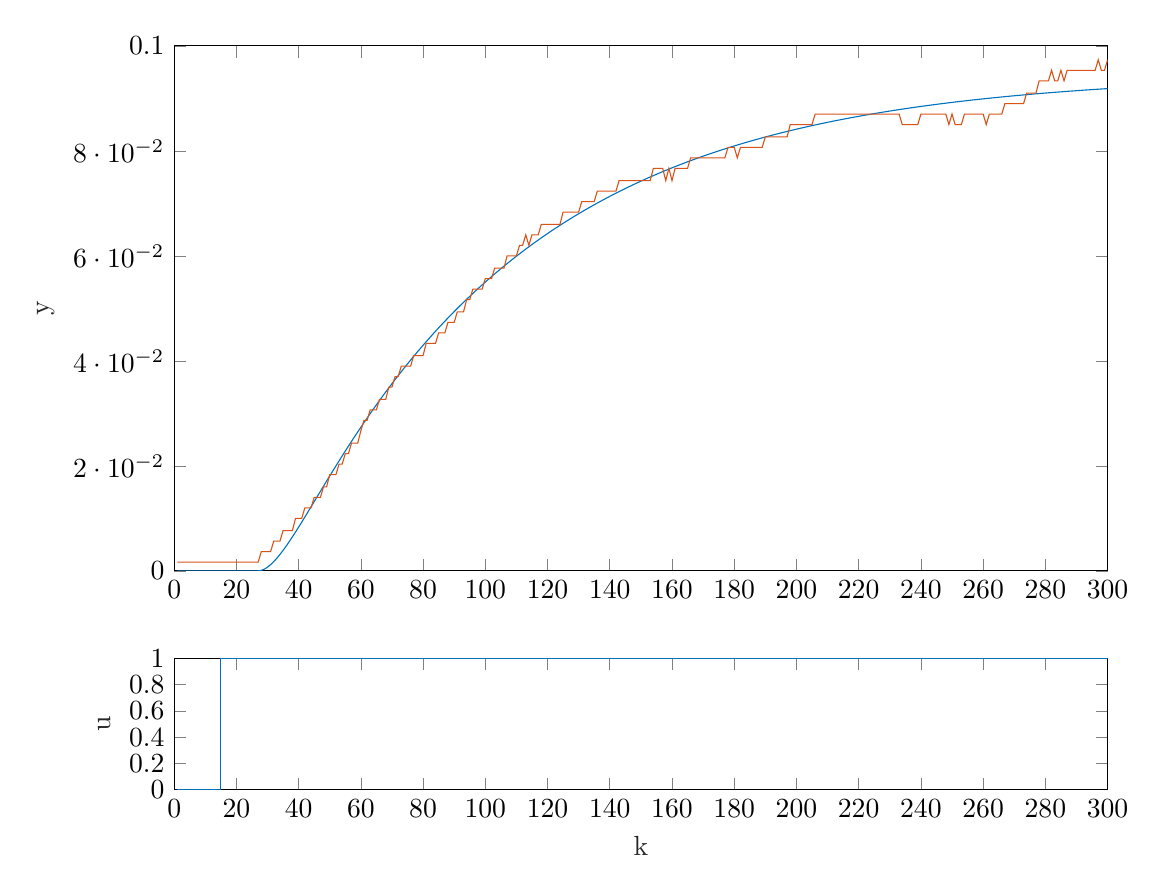
\begin{tikzpicture}

\begin{axis}[%
width=4.667in,
height=0.656in,
at={(0.583in,0.525in)},
scale only axis,
xmin=0,
xmax=300,
xlabel style={font=\color{white!15!black}},
xlabel={k},
ymin=0,
ymax=1,
ylabel style={font=\color{white!15!black}},
ylabel={u},
axis background/.style={fill=white}
]
\addplot[const plot, color=mycolor1, forget plot] table[row sep=crcr] {%
1	0\\
2	0\\
3	0\\
4	0\\
5	0\\
6	0\\
7	0\\
8	0\\
9	0\\
10	0\\
11	0\\
12	0\\
13	0\\
14	0\\
15	1\\
16	1\\
17	1\\
18	1\\
19	1\\
20	1\\
21	1\\
22	1\\
23	1\\
24	1\\
25	1\\
26	1\\
27	1\\
28	1\\
29	1\\
30	1\\
31	1\\
32	1\\
33	1\\
34	1\\
35	1\\
36	1\\
37	1\\
38	1\\
39	1\\
40	1\\
41	1\\
42	1\\
43	1\\
44	1\\
45	1\\
46	1\\
47	1\\
48	1\\
49	1\\
50	1\\
51	1\\
52	1\\
53	1\\
54	1\\
55	1\\
56	1\\
57	1\\
58	1\\
59	1\\
60	1\\
61	1\\
62	1\\
63	1\\
64	1\\
65	1\\
66	1\\
67	1\\
68	1\\
69	1\\
70	1\\
71	1\\
72	1\\
73	1\\
74	1\\
75	1\\
76	1\\
77	1\\
78	1\\
79	1\\
80	1\\
81	1\\
82	1\\
83	1\\
84	1\\
85	1\\
86	1\\
87	1\\
88	1\\
89	1\\
90	1\\
91	1\\
92	1\\
93	1\\
94	1\\
95	1\\
96	1\\
97	1\\
98	1\\
99	1\\
100	1\\
101	1\\
102	1\\
103	1\\
104	1\\
105	1\\
106	1\\
107	1\\
108	1\\
109	1\\
110	1\\
111	1\\
112	1\\
113	1\\
114	1\\
115	1\\
116	1\\
117	1\\
118	1\\
119	1\\
120	1\\
121	1\\
122	1\\
123	1\\
124	1\\
125	1\\
126	1\\
127	1\\
128	1\\
129	1\\
130	1\\
131	1\\
132	1\\
133	1\\
134	1\\
135	1\\
136	1\\
137	1\\
138	1\\
139	1\\
140	1\\
141	1\\
142	1\\
143	1\\
144	1\\
145	1\\
146	1\\
147	1\\
148	1\\
149	1\\
150	1\\
151	1\\
152	1\\
153	1\\
154	1\\
155	1\\
156	1\\
157	1\\
158	1\\
159	1\\
160	1\\
161	1\\
162	1\\
163	1\\
164	1\\
165	1\\
166	1\\
167	1\\
168	1\\
169	1\\
170	1\\
171	1\\
172	1\\
173	1\\
174	1\\
175	1\\
176	1\\
177	1\\
178	1\\
179	1\\
180	1\\
181	1\\
182	1\\
183	1\\
184	1\\
185	1\\
186	1\\
187	1\\
188	1\\
189	1\\
190	1\\
191	1\\
192	1\\
193	1\\
194	1\\
195	1\\
196	1\\
197	1\\
198	1\\
199	1\\
200	1\\
201	1\\
202	1\\
203	1\\
204	1\\
205	1\\
206	1\\
207	1\\
208	1\\
209	1\\
210	1\\
211	1\\
212	1\\
213	1\\
214	1\\
215	1\\
216	1\\
217	1\\
218	1\\
219	1\\
220	1\\
221	1\\
222	1\\
223	1\\
224	1\\
225	1\\
226	1\\
227	1\\
228	1\\
229	1\\
230	1\\
231	1\\
232	1\\
233	1\\
234	1\\
235	1\\
236	1\\
237	1\\
238	1\\
239	1\\
240	1\\
241	1\\
242	1\\
243	1\\
244	1\\
245	1\\
246	1\\
247	1\\
248	1\\
249	1\\
250	1\\
251	1\\
252	1\\
253	1\\
254	1\\
255	1\\
256	1\\
257	1\\
258	1\\
259	1\\
260	1\\
261	1\\
262	1\\
263	1\\
264	1\\
265	1\\
266	1\\
267	1\\
268	1\\
269	1\\
270	1\\
271	1\\
272	1\\
273	1\\
274	1\\
275	1\\
276	1\\
277	1\\
278	1\\
279	1\\
280	1\\
281	1\\
282	1\\
283	1\\
284	1\\
285	1\\
286	1\\
287	1\\
288	1\\
289	1\\
290	1\\
291	1\\
292	1\\
293	1\\
294	1\\
295	1\\
296	1\\
297	1\\
298	1\\
299	1\\
300	1\\
};
\end{axis}

\begin{axis}[%
width=4.667in,
height=2.625in,
at={(0.583in,1.619in)},
scale only axis,
xmin=0,
xmax=300,
ymin=0,
ymax=0.1,
ylabel style={font=\color{white!15!black}},
ylabel={y},
axis background/.style={fill=white}
]
\addplot [color=mycolor1, forget plot]
  table[row sep=crcr]{%
1	0\\
2	0\\
3	0\\
4	0\\
5	0\\
6	0\\
7	0\\
8	0\\
9	0\\
10	0\\
11	0\\
12	0\\
13	0\\
14	0\\
15	0\\
16	0\\
17	0\\
18	0\\
19	0\\
20	0\\
21	0\\
22	0\\
23	0\\
24	0\\
25	0\\
26	0\\
27	0\\
28	8.46657677711817e-05\\
29	0.000322071780209297\\
30	0.000689841089121847\\
31	0.00116858701633257\\
32	0.00174151698766157\\
33	0.00239408880822118\\
34	0.00311371243785129\\
35	0.00388949124424984\\
36	0.00471199750848349\\
37	0.00557307764918471\\
38	0.00646568323182034\\
39	0.00738372435006904\\
40	0.00832194241808434\\
41	0.00927579980436696\\
42	0.0102413840780393\\
43	0.0112153249333729\\
44	0.0121947221144226\\
45	0.013177082883743\\
46	0.0141602677718793\\
47	0.0151424435115385\\
48	0.0161220422054254\\
49	0.0170977259026053\\
50	0.0180683558674683\\
51	0.0190329659201357\\
52	0.0199907393093591\\
53	0.0209409886503055\\
54	0.0218831385215087\\
55	0.0228167103689742\\
56	0.0237413094120124\\
57	0.0246566132858058\\
58	0.0255623621907898\\
59	0.026458350349357\\
60	0.0273444185968046\\
61	0.0282204479563495\\
62	0.0290863540679163\\
63	0.0299420823576492\\
64	0.0307876038500603\\
65	0.0316229115377151\\
66	0.0324480172346134\\
67	0.0332629488492058\\
68	0.0340677480214581\\
69	0.0348624680757399\\
70	0.0356471722476929\\
71	0.0364219321487762\\
72	0.0371868264369906\\
73	0.0379419396664522\\
74	0.0386873612921054\\
75	0.0394231848090034\\
76	0.0401495070083072\\
77	0.0408664273345173\\
78	0.0415740473305034\\
79	0.0422724701586747\\
80	0.0429618001881774\\
81	0.0436421426393456\\
82	0.0443136032777934\\
83	0.0449762881515422\\
84	0.0456303033654554\\
85	0.0462757548880085\\
86	0.0469127483860813\\
87	0.0475413890840327\\
88	0.0481617816438107\\
89	0.0487740300632828\\
90	0.0493782375903436\\
91	0.0499745066506819\\
92	0.0505629387873671\\
93	0.0511436346106634\\
94	0.0517166937566859\\
95	0.0522822148537017\\
96	0.052840295495034\\
97	0.053391032217667\\
98	0.0539345204857704\\
99	0.0544708546784639\\
100	0.0550001280812325\\
101	0.0555224328804851\\
102	0.0560378601608114\\
103	0.0565464999045552\\
104	0.0570484409933718\\
105	0.0575437712114802\\
106	0.0580325772503632\\
107	0.0585149447146958\\
108	0.0589909581293181\\
109	0.059460700947088\\
110	0.0599242555574745\\
111	0.0603817032957703\\
112	0.0608331244528183\\
113	0.0612785982851603\\
114	0.0617182030255316\\
115	0.0621520158936311\\
116	0.0625801131071103\\
117	0.063002569892729\\
118	0.0634194604976362\\
119	0.0638308582007363\\
120	0.0642368353241106\\
121	0.0646374632444644\\
122	0.0650328124045778\\
123	0.065422952324738\\
124	0.0658079516141371\\
125	0.06618787798222\\
126	0.0665627982499694\\
127	0.0669327783611184\\
128	0.0672978833932801\\
129	0.067658177568988\\
130	0.0680137242666394\\
131	0.0683645860313385\\
132	0.0687108245856332\\
133	0.0690525008401423\\
134	0.0693896749040713\\
135	0.0697224060956134\\
136	0.0700507529522348\\
137	0.0703747732408424\\
138	0.0706945239678338\\
139	0.0710100613890282\\
140	0.0713214410194786\\
141	0.0716287176431648\\
142	0.0719319453225683\\
143	0.0722311774081279\\
144	0.0725264665475781\\
145	0.0728178646951703\\
146	0.073105423120777\\
147	0.0733891924188815\\
148	0.0736692225174517\\
149	0.0739455626867015\\
150	0.0742182615477386\\
151	0.0744873670811016\\
152	0.0747529266351865\\
153	0.0750149869345638\\
154	0.0752735940881883\\
155	0.0755287935975013\\
156	0.0757806303644282\\
157	0.0760291486992707\\
158	0.0762743923284968\\
159	0.0765164044024289\\
160	0.0767552275028305\\
161	0.0769909036503947\\
162	0.0772234743121334\\
163	0.0774529804086707\\
164	0.0776794623214392\\
165	0.0779029598997837\\
166	0.0781235124679695\\
167	0.0783411588321005\\
168	0.0785559372869448\\
169	0.0787678856226718\\
170	0.0789770411314999\\
171	0.079183440614257\\
172	0.0793871203868547\\
173	0.0795881162866772\\
174	0.0797864636788866\\
175	0.0799821974626443\\
176	0.0801753520772511\\
177	0.0803659615082065\\
178	0.080554059293188\\
179	0.0807396785279518\\
180	0.0809228518721552\\
181	0.0811036115551036\\
182	0.0812819893814202\\
183	0.0814580167366426\\
184	0.0816317245927443\\
185	0.0818031435135843\\
186	0.0819723036602848\\
187	0.0821392347965378\\
188	0.0823039662938418\\
189	0.0824665271366701\\
190	0.0826269459275698\\
191	0.082785250892195\\
192	0.0829414698842727\\
193	0.0830956303905039\\
194	0.0832477595353995\\
195	0.083397884086053\\
196	0.0835460304568501\\
197	0.0836922247141164\\
198	0.0838364925807035\\
199	0.083978859440515\\
200	0.084119350342973\\
201	0.0842579900074254\\
202	0.0843948028274948\\
203	0.0845298128753713\\
204	0.0846630439060476\\
205	0.0847945193614986\\
206	0.0849242623748061\\
207	0.0850522957742291\\
208	0.0851786420872205\\
209	0.0853033235443906\\
210	0.0854263620834185\\
211	0.0855477793529124\\
212	0.0856675967162184\\
213	0.0857858352551794\\
214	0.0859025157738443\\
215	0.0860176588021289\\
216	0.0861312845994276\\
217	0.0862434131581787\\
218	0.0863540642073811\\
219	0.0864632572160667\\
220	0.086571011396725\\
221	0.0866773457086844\\
222	0.0867822788614474\\
223	0.0868858293179828\\
224	0.0869880152979745\\
225	0.0870888547810266\\
226	0.0871883655098277\\
227	0.0872865649932721\\
228	0.0873834705095408\\
229	0.0874790991091416\\
230	0.0875734676179089\\
231	0.0876665926399645\\
232	0.0877584905606387\\
233	0.087849177549354\\
234	0.087938669562469\\
235	0.0880269823460872\\
236	0.0881141314388265\\
237	0.0882001321745537\\
238	0.0882849996850824\\
239	0.0883687489028354\\
240	0.0884513945634722\\
241	0.0885329512084815\\
242	0.0886134331877401\\
243	0.0886928546620372\\
244	0.0887712296055668\\
245	0.0888485718083855\\
246	0.0889248948788399\\
247	0.0890002122459601\\
248	0.0890745371618228\\
249	0.0891478827038835\\
250	0.0892202617772767\\
251	0.089291687117087\\
252	0.0893621712905899\\
253	0.0894317266994626\\
254	0.0895003655819665\\
255	0.0895681000151004\\
256	0.0896349419167252\\
257	0.0897009030476614\\
258	0.0897659950137576\\
259	0.0898302292679334\\
260	0.0898936171121939\\
261	0.0899561696996187\\
262	0.0900178980363239\\
263	0.0900788129833991\\
264	0.0901389252588179\\
265	0.0901982454393242\\
266	0.0902567839622928\\
267	0.090314551127566\\
268	0.0903715570992659\\
269	0.0904278119075827\\
270	0.0904833254505396\\
271	0.0905381074957342\\
272	0.0905921676820573\\
273	0.0906455155213888\\
274	0.090698160400271\\
275	0.0907501115815608\\
276	0.090801378206059\\
277	0.0908519692941186\\
278	0.0909018937472323\\
279	0.0909511603495985\\
280	0.0909997777696666\\
281	0.0910477545616629\\
282	0.091095099167095\\
283	0.0911418199162376\\
284	0.0911879250295979\\
285	0.091233422619362\\
286	0.0912783206908225\\
287	0.0913226271437867\\
288	0.091366349773967\\
289	0.091409496274352\\
290	0.0914520742365606\\
291	0.0914940911521773\\
292	0.0915355544140708\\
293	0.0915764713176942\\
294	0.0916168490623693\\
295	0.0916566947525528\\
296	0.0916960153990866\\
297	0.0917348179204311\\
298	0.0917731091438828\\
299	0.0918108958067755\\
300	0.0918481845576655\\
};
\addplot [color=mycolor2, forget plot]
  table[row sep=crcr]{%
1	0.00166666666666657\\
2	0.00166666666666657\\
3	0.00166666666666657\\
4	0.00166666666666657\\
5	0.00166666666666657\\
6	0.00166666666666657\\
7	0.00166666666666657\\
8	0.00166666666666657\\
9	0.00166666666666657\\
10	0.00166666666666657\\
11	0.00166666666666657\\
12	0.00166666666666657\\
13	0.00166666666666657\\
14	0.00166666666666657\\
15	0.00166666666666657\\
16	0.00166666666666657\\
17	0.00166666666666657\\
18	0.00166666666666657\\
19	0.00166666666666657\\
20	0.00166666666666657\\
21	0.00166666666666657\\
22	0.00166666666666657\\
23	0.00166666666666657\\
24	0.00166666666666657\\
25	0.00166666666666657\\
26	0.00166666666666657\\
27	0.00166666666666657\\
28	0.00366666666666665\\
29	0.00366666666666665\\
30	0.00366666666666665\\
31	0.00366666666666665\\
32	0.00566666666666649\\
33	0.00566666666666649\\
34	0.00566666666666649\\
35	0.00766666666666656\\
36	0.00766666666666656\\
37	0.00766666666666656\\
38	0.00766666666666656\\
39	0.0099999999999999\\
40	0.0099999999999999\\
41	0.0099999999999999\\
42	0.012\\
43	0.012\\
44	0.012\\
45	0.0139999999999998\\
46	0.0139999999999998\\
47	0.0139999999999998\\
48	0.0159999999999999\\
49	0.0159999999999999\\
50	0.0183333333333332\\
51	0.0183333333333332\\
52	0.0183333333333332\\
53	0.0203333333333333\\
54	0.0203333333333333\\
55	0.0223333333333332\\
56	0.0223333333333332\\
57	0.0243333333333332\\
58	0.0243333333333332\\
59	0.0243333333333332\\
60	0.0266666666666666\\
61	0.0286666666666666\\
62	0.0286666666666666\\
63	0.0306666666666665\\
64	0.0306666666666665\\
65	0.0306666666666665\\
66	0.0326666666666666\\
67	0.0326666666666666\\
68	0.0326666666666666\\
69	0.0349999999999999\\
70	0.0349999999999999\\
71	0.037\\
72	0.037\\
73	0.0389999999999998\\
74	0.0389999999999998\\
75	0.0389999999999998\\
76	0.0389999999999998\\
77	0.0409999999999999\\
78	0.0409999999999999\\
79	0.0409999999999999\\
80	0.0409999999999999\\
81	0.0433333333333332\\
82	0.0433333333333332\\
83	0.0433333333333332\\
84	0.0433333333333332\\
85	0.0453333333333333\\
86	0.0453333333333333\\
87	0.0453333333333333\\
88	0.0473333333333332\\
89	0.0473333333333332\\
90	0.0473333333333332\\
91	0.0493333333333332\\
92	0.0493333333333332\\
93	0.0493333333333332\\
94	0.0516666666666666\\
95	0.0516666666666666\\
96	0.0536666666666666\\
97	0.0536666666666666\\
98	0.0536666666666666\\
99	0.0536666666666666\\
100	0.0556666666666665\\
101	0.0556666666666665\\
102	0.0556666666666665\\
103	0.0576666666666666\\
104	0.0576666666666666\\
105	0.0576666666666666\\
106	0.0576666666666666\\
107	0.0599999999999999\\
108	0.0599999999999999\\
109	0.0599999999999999\\
110	0.0599999999999999\\
111	0.062\\
112	0.062\\
113	0.0639999999999998\\
114	0.062\\
115	0.0639999999999998\\
116	0.0639999999999998\\
117	0.0639999999999998\\
118	0.0659999999999999\\
119	0.0659999999999999\\
120	0.0659999999999999\\
121	0.0659999999999999\\
122	0.0659999999999999\\
123	0.0659999999999999\\
124	0.0659999999999999\\
125	0.0683333333333332\\
126	0.0683333333333332\\
127	0.0683333333333332\\
128	0.0683333333333332\\
129	0.0683333333333332\\
130	0.0683333333333332\\
131	0.0703333333333333\\
132	0.0703333333333333\\
133	0.0703333333333333\\
134	0.0703333333333333\\
135	0.0703333333333333\\
136	0.0723333333333332\\
137	0.0723333333333332\\
138	0.0723333333333332\\
139	0.0723333333333332\\
140	0.0723333333333332\\
141	0.0723333333333332\\
142	0.0723333333333332\\
143	0.0743333333333332\\
144	0.0743333333333332\\
145	0.0743333333333332\\
146	0.0743333333333332\\
147	0.0743333333333332\\
148	0.0743333333333332\\
149	0.0743333333333332\\
150	0.0743333333333332\\
151	0.0743333333333332\\
152	0.0743333333333332\\
153	0.0743333333333332\\
154	0.0766666666666666\\
155	0.0766666666666666\\
156	0.0766666666666666\\
157	0.0766666666666666\\
158	0.0743333333333332\\
159	0.0766666666666666\\
160	0.0743333333333332\\
161	0.0766666666666666\\
162	0.0766666666666666\\
163	0.0766666666666666\\
164	0.0766666666666666\\
165	0.0766666666666666\\
166	0.0786666666666666\\
167	0.0786666666666666\\
168	0.0786666666666666\\
169	0.0786666666666666\\
170	0.0786666666666666\\
171	0.0786666666666666\\
172	0.0786666666666666\\
173	0.0786666666666666\\
174	0.0786666666666666\\
175	0.0786666666666666\\
176	0.0786666666666666\\
177	0.0786666666666666\\
178	0.0806666666666665\\
179	0.0806666666666665\\
180	0.0806666666666665\\
181	0.0786666666666666\\
182	0.0806666666666665\\
183	0.0806666666666665\\
184	0.0806666666666665\\
185	0.0806666666666665\\
186	0.0806666666666665\\
187	0.0806666666666665\\
188	0.0806666666666665\\
189	0.0806666666666665\\
190	0.0826666666666666\\
191	0.0826666666666666\\
192	0.0826666666666666\\
193	0.0826666666666666\\
194	0.0826666666666666\\
195	0.0826666666666666\\
196	0.0826666666666666\\
197	0.0826666666666666\\
198	0.0849999999999999\\
199	0.0849999999999999\\
200	0.0849999999999999\\
201	0.0849999999999999\\
202	0.0849999999999999\\
203	0.0849999999999999\\
204	0.0849999999999999\\
205	0.0849999999999999\\
206	0.087\\
207	0.087\\
208	0.087\\
209	0.087\\
210	0.087\\
211	0.087\\
212	0.087\\
213	0.087\\
214	0.087\\
215	0.087\\
216	0.087\\
217	0.087\\
218	0.087\\
219	0.087\\
220	0.087\\
221	0.087\\
222	0.087\\
223	0.087\\
224	0.087\\
225	0.087\\
226	0.087\\
227	0.087\\
228	0.087\\
229	0.087\\
230	0.087\\
231	0.087\\
232	0.087\\
233	0.087\\
234	0.0849999999999999\\
235	0.0849999999999999\\
236	0.0849999999999999\\
237	0.0849999999999999\\
238	0.0849999999999999\\
239	0.0849999999999999\\
240	0.087\\
241	0.087\\
242	0.087\\
243	0.087\\
244	0.087\\
245	0.087\\
246	0.087\\
247	0.087\\
248	0.087\\
249	0.0849999999999999\\
250	0.087\\
251	0.0849999999999999\\
252	0.0849999999999999\\
253	0.0849999999999999\\
254	0.087\\
255	0.087\\
256	0.087\\
257	0.087\\
258	0.087\\
259	0.087\\
260	0.087\\
261	0.0849999999999999\\
262	0.087\\
263	0.087\\
264	0.087\\
265	0.087\\
266	0.087\\
267	0.0889999999999998\\
268	0.0889999999999998\\
269	0.0889999999999998\\
270	0.0889999999999998\\
271	0.0889999999999998\\
272	0.0889999999999998\\
273	0.0889999999999998\\
274	0.0909999999999999\\
275	0.0909999999999999\\
276	0.0909999999999999\\
277	0.0909999999999999\\
278	0.0933333333333332\\
279	0.0933333333333332\\
280	0.0933333333333332\\
281	0.0933333333333332\\
282	0.0953333333333333\\
283	0.0933333333333332\\
284	0.0933333333333332\\
285	0.0953333333333333\\
286	0.0933333333333332\\
287	0.0953333333333333\\
288	0.0953333333333333\\
289	0.0953333333333333\\
290	0.0953333333333333\\
291	0.0953333333333333\\
292	0.0953333333333333\\
293	0.0953333333333333\\
294	0.0953333333333333\\
295	0.0953333333333333\\
296	0.0953333333333333\\
297	0.0973333333333331\\
298	0.0953333333333333\\
299	0.0953333333333333\\
300	0.0973333333333331\\
};
\end{axis}
\end{tikzpicture}%
\caption{Aproksymacja modelu dla wybranego skoku zakłóceń}
\label{R3}
\end{figure}

\begin{figure}[ht]
\centering
% This file was created by matlab2tikz.
%
%The latest updates can be retrieved from
%  http://www.mathworks.com/matlabcentral/fileexchange/22022-matlab2tikz-matlab2tikz
%where you can also make suggestions and rate matlab2tikz.
%
\definecolor{mycolor1}{rgb}{0.00000,0.44700,0.74100}%
%
\begin{tikzpicture}

\begin{axis}[%
width=4.521in,
height=3.566in,
at={(0.758in,0.481in)},
scale only axis,
xmin=0,
xmax=300,
xtick={0,50,100,150,200,250,300},
xlabel style={font=\color{white!15!black}},
xlabel={k},
ymin=0,
ymax=0.1,
ytick={0,0.01,0.02,0.03,0.04,0.05,0.06,0.07,0.08,0.09,0.1},
yticklabels={{0},{0,01},{0,02},{0,03},{0,04},{0,05},{0,06},{0,07},{0,08},{0,09},{0,1}},
ylabel style={font=\color{white!15!black}},
ylabel={s},
axis background/.style={fill=white}
]
\addplot[const plot, color=mycolor1, forget plot] table[row sep=crcr] {%
1	0\\
2	0\\
3	0\\
4	0\\
5	0\\
6	0\\
7	0\\
8	0\\
9	0\\
10	0\\
11	0\\
12	0\\
13	0\\
14	0\\
15	0\\
16	8.4666e-05\\
17	0.00032207\\
18	0.00068984\\
19	0.0011686\\
20	0.0017415\\
21	0.0023941\\
22	0.0031137\\
23	0.0038895\\
24	0.004712\\
25	0.0055731\\
26	0.0064657\\
27	0.0073837\\
28	0.0083219\\
29	0.0092758\\
30	0.010241\\
31	0.011215\\
32	0.012195\\
33	0.013177\\
34	0.01416\\
35	0.015142\\
36	0.016122\\
37	0.017098\\
38	0.018068\\
39	0.019033\\
40	0.019991\\
41	0.020941\\
42	0.021883\\
43	0.022817\\
44	0.023741\\
45	0.024657\\
46	0.025562\\
47	0.026458\\
48	0.027344\\
49	0.02822\\
50	0.029086\\
51	0.029942\\
52	0.030788\\
53	0.031623\\
54	0.032448\\
55	0.033263\\
56	0.034068\\
57	0.034862\\
58	0.035647\\
59	0.036422\\
60	0.037187\\
61	0.037942\\
62	0.038687\\
63	0.039423\\
64	0.04015\\
65	0.040866\\
66	0.041574\\
67	0.042272\\
68	0.042962\\
69	0.043642\\
70	0.044314\\
71	0.044976\\
72	0.04563\\
73	0.046276\\
74	0.046913\\
75	0.047541\\
76	0.048162\\
77	0.048774\\
78	0.049378\\
79	0.049975\\
80	0.050563\\
81	0.051144\\
82	0.051717\\
83	0.052282\\
84	0.05284\\
85	0.053391\\
86	0.053935\\
87	0.054471\\
88	0.055\\
89	0.055522\\
90	0.056038\\
91	0.056546\\
92	0.057048\\
93	0.057544\\
94	0.058033\\
95	0.058515\\
96	0.058991\\
97	0.059461\\
98	0.059924\\
99	0.060382\\
100	0.060833\\
101	0.061279\\
102	0.061718\\
103	0.062152\\
104	0.06258\\
105	0.063003\\
106	0.063419\\
107	0.063831\\
108	0.064237\\
109	0.064637\\
110	0.065033\\
111	0.065423\\
112	0.065808\\
113	0.066188\\
114	0.066563\\
115	0.066933\\
116	0.067298\\
117	0.067658\\
118	0.068014\\
119	0.068365\\
120	0.068711\\
121	0.069053\\
122	0.06939\\
123	0.069722\\
124	0.070051\\
125	0.070375\\
126	0.070695\\
127	0.07101\\
128	0.071321\\
129	0.071629\\
130	0.071932\\
131	0.072231\\
132	0.072526\\
133	0.072818\\
134	0.073105\\
135	0.073389\\
136	0.073669\\
137	0.073946\\
138	0.074218\\
139	0.074487\\
140	0.074753\\
141	0.075015\\
142	0.075274\\
143	0.075529\\
144	0.075781\\
145	0.076029\\
146	0.076274\\
147	0.076516\\
148	0.076755\\
149	0.076991\\
150	0.077223\\
151	0.077453\\
152	0.077679\\
153	0.077903\\
154	0.078124\\
155	0.078341\\
156	0.078556\\
157	0.078768\\
158	0.078977\\
159	0.079183\\
160	0.079387\\
161	0.079588\\
162	0.079786\\
163	0.079982\\
164	0.080175\\
165	0.080366\\
166	0.080554\\
167	0.08074\\
168	0.080923\\
169	0.081104\\
170	0.081282\\
171	0.081458\\
172	0.081632\\
173	0.081803\\
174	0.081972\\
175	0.082139\\
176	0.082304\\
177	0.082467\\
178	0.082627\\
179	0.082785\\
180	0.082941\\
181	0.083096\\
182	0.083248\\
183	0.083398\\
184	0.083546\\
185	0.083692\\
186	0.083836\\
187	0.083979\\
188	0.084119\\
189	0.084258\\
190	0.084395\\
191	0.08453\\
192	0.084663\\
193	0.084795\\
194	0.084924\\
195	0.085052\\
196	0.085179\\
197	0.085303\\
198	0.085426\\
199	0.085548\\
200	0.085668\\
201	0.085786\\
202	0.085903\\
203	0.086018\\
204	0.086131\\
205	0.086243\\
206	0.086354\\
207	0.086463\\
208	0.086571\\
209	0.086677\\
210	0.086782\\
211	0.086886\\
212	0.086988\\
213	0.087089\\
214	0.087188\\
215	0.087287\\
216	0.087383\\
217	0.087479\\
218	0.087573\\
219	0.087667\\
220	0.087758\\
221	0.087849\\
222	0.087939\\
223	0.088027\\
224	0.088114\\
225	0.0882\\
226	0.088285\\
227	0.088369\\
228	0.088451\\
229	0.088533\\
230	0.088613\\
231	0.088693\\
232	0.088771\\
233	0.088849\\
234	0.088925\\
235	0.089\\
236	0.089075\\
237	0.089148\\
238	0.08922\\
239	0.089292\\
240	0.089362\\
241	0.089432\\
242	0.0895\\
243	0.089568\\
244	0.089635\\
245	0.089701\\
246	0.089766\\
247	0.08983\\
248	0.089894\\
249	0.089956\\
250	0.090018\\
251	0.090079\\
252	0.090139\\
253	0.090198\\
254	0.090257\\
255	0.090315\\
256	0.090372\\
257	0.090428\\
258	0.090483\\
259	0.090538\\
260	0.090592\\
261	0.090646\\
262	0.090698\\
263	0.09075\\
264	0.090801\\
265	0.090852\\
266	0.090902\\
267	0.090951\\
268	0.091\\
269	0.091048\\
270	0.091095\\
271	0.091142\\
272	0.091188\\
273	0.091233\\
274	0.091278\\
275	0.091323\\
276	0.091366\\
277	0.091409\\
278	0.091452\\
279	0.091494\\
280	0.091536\\
281	0.091576\\
282	0.091617\\
283	0.091657\\
284	0.091696\\
285	0.091735\\
286	0.091773\\
287	0.091811\\
288	0.091848\\
};
\end{axis}
\end{tikzpicture}%
\caption{Zamodelowana, poprawna odpowiedź obiektu na skok zakłócenia}
\label{R4}
\end{figure}

\begin{figure}[ht]
\centering
% This file was created by matlab2tikz.
%
%The latest updates can be retrieved from
%  http://www.mathworks.com/matlabcentral/fileexchange/22022-matlab2tikz-matlab2tikz
%where you can also make suggestions and rate matlab2tikz.
%
\definecolor{mycolor1}{rgb}{0.00000,0.44700,0.74100}%
%
\begin{tikzpicture}

\begin{axis}[%
width=4.521in,
height=3.566in,
at={(0.758in,0.481in)},
scale only axis,
xmin=0,
xmax=400,
xtick={0,50,100,150,200,250,300,350,400},
xlabel style={font=\color{white!15!black}},
xlabel={$k$},
ymin=0,
ymax=0.3,
ytick={0,0.05,0.1,0.15,0.2,0.25,0.3},
yticklabels={{0},{0,05},{0,1},{0,15},{0,2},{0,25},{0,3}},
ylabel style={font=\color{white!15!black}},
ylabel={$s_i$},
axis background/.style={fill=white}
]
\addplot[const plot, color=mycolor1, forget plot] table[row sep=crcr] {%
1	0\\
27	0.00306110000002491\\
28	0.00608940000000757\\
29	0.00908509999999296\\
30	0.0120489999999904\\
31	0.01497999999998\\
32	0.0178809999999885\\
33	0.0207500000000209\\
34	0.0235880000000179\\
35	0.026395999999977\\
36	0.0291740000000118\\
37	0.0319210000000112\\
38	0.0346400000000244\\
39	0.0373289999999997\\
40	0.0399889999999914\\
41	0.0426209999999969\\
42	0.0452240000000188\\
43	0.0477989999999977\\
44	0.0503469999999879\\
45	0.0528679999999895\\
46	0.0553610000000049\\
47	0.0578269999999748\\
48	0.0602680000000078\\
49	0.0626809999999978\\
50	0.065068999999994\\
51	0.0674319999999966\\
52	0.069769000000008\\
53	0.0720800000000281\\
54	0.0743669999999952\\
55	0.0766300000000228\\
56	0.0788679999999999\\
57	0.0810819999999808\\
58	0.0832720000000222\\
59	0.085439000000008\\
60	0.0875829999999951\\
61	0.0897029999999859\\
62	0.0918009999999754\\
63	0.0938760000000229\\
64	0.0959290000000124\\
65	0.0979600000000005\\
66	0.0999689999999873\\
67	0.10196000000002\\
68	0.103920000000016\\
69	0.105869999999982\\
70	0.107790000000023\\
71	0.109690000000001\\
72	0.111580000000004\\
73	0.113440000000026\\
74	0.115279999999984\\
75	0.117110000000025\\
76	0.118910000000028\\
77	0.120690000000025\\
78	0.12245999999999\\
79	0.124199999999973\\
80	0.125929999999983\\
81	0.127639999999985\\
82	0.129329999999982\\
83	0.130999999999972\\
84	0.132659999999987\\
85	0.134290000000021\\
86	0.135910000000024\\
87	0.13751000000002\\
88	0.139099999999985\\
89	0.140660000000025\\
90	0.142220000000009\\
91	0.143750000000011\\
92	0.145269999999982\\
93	0.146770000000004\\
94	0.148250000000019\\
95	0.149720000000002\\
96	0.151169999999979\\
97	0.152609999999981\\
98	0.154029999999977\\
99	0.155439999999999\\
100	0.156830000000014\\
101	0.158209999999997\\
102	0.159569999999974\\
103	0.160919999999976\\
104	0.162249999999972\\
105	0.163569999999993\\
106	0.164870000000008\\
107	0.166159999999991\\
108	0.167439999999999\\
109	0.168700000000001\\
110	0.169949999999972\\
111	0.171190000000024\\
112	0.172410000000014\\
113	0.173620000000028\\
114	0.174820000000011\\
115	0.175999999999988\\
116	0.17716999999999\\
117	0.178330000000017\\
118	0.179480000000012\\
119	0.180610000000001\\
120	0.181730000000016\\
121	0.182839999999999\\
122	0.183940000000007\\
123	0.185020000000009\\
124	0.18610000000001\\
125	0.187160000000006\\
126	0.188210000000026\\
127	0.189250000000015\\
128	0.190279999999973\\
129	0.191300000000012\\
130	0.192299999999989\\
131	0.193300000000022\\
132	0.194279999999992\\
133	0.195260000000019\\
134	0.196219999999983\\
135	0.197180000000003\\
136	0.198120000000017\\
137	0.19905\\
138	0.199979999999982\\
139	0.200890000000015\\
140	0.201790000000017\\
141	0.202690000000018\\
142	0.203570000000013\\
143	0.204450000000008\\
144	0.205309999999997\\
145	0.206169999999986\\
146	0.207010000000025\\
147	0.207850000000008\\
148	0.208680000000015\\
149	0.209499999999991\\
150	0.210309999999993\\
151	0.211110000000019\\
152	0.211909999999989\\
153	0.212690000000009\\
154	0.213469999999973\\
155	0.214240000000018\\
156	0.214999999999975\\
157	0.215750000000014\\
158	0.216490000000022\\
159	0.217229999999972\\
160	0.217960000000005\\
161	0.218680000000006\\
162	0.219389999999976\\
163	0.220100000000002\\
164	0.220790000000022\\
165	0.221479999999985\\
166	0.222159999999974\\
167	0.222840000000019\\
168	0.223509999999976\\
169	0.224170000000015\\
170	0.224820000000022\\
171	0.225469999999973\\
172	0.226110000000006\\
173	0.226740000000007\\
174	0.227370000000008\\
175	0.227989999999977\\
176	0.228599999999972\\
177	0.229199999999992\\
178	0.229800000000012\\
179	0.230399999999975\\
180	0.230979999999988\\
181	0.231560000000002\\
182	0.232140000000015\\
183	0.232709999999997\\
184	0.233270000000005\\
185	0.23381999999998\\
186	0.234370000000013\\
187	0.234919999999988\\
188	0.235450000000014\\
189	0.235990000000015\\
190	0.23651000000001\\
191	0.237030000000004\\
192	0.237549999999999\\
193	0.238060000000019\\
194	0.238560000000007\\
195	0.239059999999995\\
196	0.239559999999983\\
197	0.240040000000022\\
198	0.240529999999978\\
199	0.241010000000017\\
200	0.241480000000024\\
201	0.241949999999974\\
202	0.242410000000007\\
203	0.242869999999982\\
204	0.243319999999983\\
205	0.243769999999984\\
206	0.24421000000001\\
207	0.244649999999979\\
208	0.245079999999973\\
209	0.245510000000024\\
210	0.245929999999987\\
211	0.246350000000007\\
212	0.246770000000026\\
213	0.247180000000014\\
214	0.247590000000002\\
215	0.247990000000016\\
216	0.248389999999972\\
217	0.248780000000011\\
218	0.249169999999992\\
219	0.249549999999999\\
220	0.249939999999981\\
221	0.250310000000013\\
222	0.250679999999988\\
223	0.251050000000021\\
224	0.251419999999996\\
225	0.251779999999997\\
226	0.252139999999997\\
227	0.252490000000023\\
228	0.252839999999992\\
229	0.253179999999986\\
230	0.253530000000012\\
231	0.253859999999975\\
232	0.254200000000026\\
233	0.254529999999988\\
234	0.254860000000008\\
235	0.255179999999996\\
236	0.255499999999984\\
237	0.255820000000028\\
238	0.256129999999985\\
239	0.256439999999998\\
240	0.256750000000011\\
241	0.257049999999992\\
242	0.257349999999974\\
243	0.257650000000012\\
244	0.257940000000019\\
245	0.258240000000001\\
246	0.258519999999976\\
247	0.258809999999983\\
248	0.259090000000015\\
249	0.25936999999999\\
250	0.25963999999999\\
251	0.259920000000022\\
252	0.260179999999991\\
253	0.260449999999992\\
254	0.260719999999992\\
255	0.260980000000018\\
256	0.261230000000012\\
257	0.261489999999981\\
258	0.261739999999975\\
259	0.261990000000026\\
260	0.26224000000002\\
261	0.262479999999982\\
262	0.262729999999976\\
263	0.262969999999996\\
264	0.263199999999983\\
265	0.263440000000003\\
266	0.263669999999991\\
267	0.263899999999978\\
268	0.264130000000023\\
269	0.264349999999979\\
270	0.264569999999992\\
271	0.264790000000005\\
272	0.265010000000018\\
273	0.265219999999999\\
274	0.265440000000012\\
275	0.265649999999994\\
276	0.26585\\
277	0.266059999999982\\
278	0.266259999999988\\
279	0.266459999999995\\
280	0.266660000000002\\
281	0.266860000000008\\
282	0.267060000000015\\
283	0.26724999999999\\
284	0.267440000000022\\
285	0.267629999999997\\
286	0.267819999999972\\
287	0.267999999999972\\
288	0.268179999999973\\
289	0.268359999999973\\
290	0.268539999999973\\
291	0.268719999999973\\
292	0.268889999999999\\
293	0.269069999999999\\
294	0.269240000000025\\
295	0.269409999999993\\
296	0.269580000000019\\
297	0.269740000000013\\
298	0.269909999999982\\
299	0.270069999999976\\
300	0.270230000000026\\
301	0.27039000000002\\
302	0.270539999999983\\
303	0.270699999999977\\
304	0.270849999999996\\
305	0.27100999999999\\
306	0.271160000000009\\
307	0.271310000000028\\
308	0.271450000000016\\
309	0.271599999999978\\
310	0.271740000000023\\
311	0.271889999999985\\
312	0.272029999999972\\
313	0.272170000000017\\
314	0.272299999999973\\
315	0.272440000000017\\
316	0.272580000000005\\
317	0.272710000000018\\
318	0.272839999999974\\
319	0.272969999999987\\
320	0.273099999999999\\
321	0.273230000000012\\
322	0.273360000000025\\
323	0.273480000000006\\
324	0.273610000000019\\
325	0.27373\\
326	0.273849999999982\\
327	0.27397000000002\\
328	0.274090000000001\\
329	0.274200000000008\\
330	0.274319999999989\\
331	0.274440000000027\\
332	0.274549999999977\\
333	0.274659999999983\\
334	0.27476999999999\\
335	0.274879999999996\\
336	0.274990000000003\\
337	0.275100000000009\\
338	0.275210000000016\\
339	0.27530999999999\\
340	0.275419999999997\\
341	0.275519999999972\\
342	0.275620000000004\\
343	0.275719999999978\\
344	0.27582000000001\\
345	0.275919999999985\\
346	0.276020000000017\\
347	0.276110000000017\\
348	0.276209999999992\\
349	0.276299999999992\\
350	0.276400000000024\\
351	0.276490000000024\\
352	0.276580000000024\\
353	0.276670000000024\\
354	0.276760000000024\\
355	0.276850000000024\\
356	0.276940000000025\\
357	0.277030000000025\\
358	0.277109999999993\\
359	0.277199999999993\\
360	0.277280000000019\\
361	0.277359999999987\\
362	0.277449999999988\\
363	0.277530000000013\\
364	0.277609999999981\\
365	0.277690000000007\\
366	0.277769999999975\\
367	0.277840000000026\\
368	0.277919999999995\\
369	0.27800000000002\\
370	0.278070000000014\\
371	0.278149999999982\\
};
\end{axis}
\end{tikzpicture}%

\caption{Zamodelowana odpowiedź obiektu na skok sterowania}
\label{R5}
\end{figure}

\begin{figure}[ht]
\centering
% This file was created by matlab2tikz.
%
%The latest updates can be retrieved from
%  http://www.mathworks.com/matlabcentral/fileexchange/22022-matlab2tikz-matlab2tikz
%where you can also make suggestions and rate matlab2tikz.
%
\definecolor{mycolor1}{rgb}{0.00000,0.44700,0.74100}%
%
\begin{tikzpicture}

\begin{axis}[%
width=4.521in,
height=3.566in,
at={(0.758in,0.481in)},
scale only axis,
xmin=0,
xmax=300,
xtick={0,50,100,150,200,250,300},
xlabel style={font=\color{white!15!black}},
xlabel={k},
ymin=0,
ymax=0.3,
ytick={0,0.05,0.1,0.15,0.2,0.25,0.3},
yticklabels={{0},{0,05},{0,1},{0,15},{0,2},{0,25},{0,3}},
ylabel style={font=\color{white!15!black}},
ylabel={y},
axis background/.style={fill=white}
]
\addplot[const plot, color=mycolor1, forget plot] table[row sep=crcr] {%
1	0\\
2	0\\
3	0\\
4	0\\
5	0\\
6	0\\
7	0\\
8	0\\
9	0\\
10	0\\
11	0\\
12	0\\
13	0\\
14	0.000254\\
15	0.00096623\\
16	0.0020695\\
17	0.0035058\\
18	0.0052246\\
19	0.0071823\\
20	0.0093412\\
21	0.011669\\
22	0.014136\\
23	0.016719\\
24	0.019397\\
25	0.022151\\
26	0.024966\\
27	0.027828\\
28	0.030724\\
29	0.033646\\
30	0.036584\\
31	0.039531\\
32	0.042481\\
33	0.045427\\
34	0.048366\\
35	0.051293\\
36	0.054205\\
37	0.057099\\
38	0.059972\\
39	0.062823\\
40	0.06565\\
41	0.06845\\
42	0.071224\\
43	0.07397\\
44	0.076687\\
45	0.079375\\
46	0.082033\\
47	0.084661\\
48	0.087259\\
49	0.089826\\
50	0.092363\\
51	0.094869\\
52	0.097344\\
53	0.099789\\
54	0.1022\\
55	0.10459\\
56	0.10694\\
57	0.10927\\
58	0.11156\\
59	0.11383\\
60	0.11606\\
61	0.11827\\
62	0.12045\\
63	0.1226\\
64	0.12472\\
65	0.12682\\
66	0.12889\\
67	0.13093\\
68	0.13294\\
69	0.13493\\
70	0.13689\\
71	0.13883\\
72	0.14074\\
73	0.14262\\
74	0.14449\\
75	0.14632\\
76	0.14813\\
77	0.14992\\
78	0.15169\\
79	0.15343\\
80	0.15515\\
81	0.15685\\
82	0.15852\\
83	0.16017\\
84	0.1618\\
85	0.16341\\
86	0.165\\
87	0.16657\\
88	0.16811\\
89	0.16964\\
90	0.17115\\
91	0.17263\\
92	0.1741\\
93	0.17554\\
94	0.17697\\
95	0.17838\\
96	0.17977\\
97	0.18115\\
98	0.1825\\
99	0.18384\\
100	0.18515\\
101	0.18646\\
102	0.18774\\
103	0.18901\\
104	0.19026\\
105	0.19149\\
106	0.19271\\
107	0.19391\\
108	0.1951\\
109	0.19627\\
110	0.19742\\
111	0.19856\\
112	0.19969\\
113	0.2008\\
114	0.20189\\
115	0.20297\\
116	0.20404\\
117	0.20509\\
118	0.20613\\
119	0.20716\\
120	0.20817\\
121	0.20917\\
122	0.21015\\
123	0.21112\\
124	0.21208\\
125	0.21303\\
126	0.21396\\
127	0.21489\\
128	0.2158\\
129	0.21669\\
130	0.21758\\
131	0.21845\\
132	0.21932\\
133	0.22017\\
134	0.22101\\
135	0.22184\\
136	0.22265\\
137	0.22346\\
138	0.22426\\
139	0.22504\\
140	0.22582\\
141	0.22659\\
142	0.22734\\
143	0.22809\\
144	0.22882\\
145	0.22955\\
146	0.23027\\
147	0.23097\\
148	0.23167\\
149	0.23236\\
150	0.23304\\
151	0.23371\\
152	0.23437\\
153	0.23502\\
154	0.23567\\
155	0.2363\\
156	0.23693\\
157	0.23755\\
158	0.23816\\
159	0.23876\\
160	0.23936\\
161	0.23995\\
162	0.24053\\
163	0.2411\\
164	0.24166\\
165	0.24222\\
166	0.24277\\
167	0.24331\\
168	0.24385\\
169	0.24437\\
170	0.2449\\
171	0.24541\\
172	0.24592\\
173	0.24642\\
174	0.24691\\
175	0.2474\\
176	0.24788\\
177	0.24836\\
178	0.24882\\
179	0.24929\\
180	0.24974\\
181	0.25019\\
182	0.25064\\
183	0.25108\\
184	0.25151\\
185	0.25194\\
186	0.25236\\
187	0.25277\\
188	0.25318\\
189	0.25359\\
190	0.25399\\
191	0.25438\\
192	0.25477\\
193	0.25516\\
194	0.25554\\
195	0.25591\\
196	0.25628\\
197	0.25664\\
198	0.257\\
199	0.25736\\
200	0.25771\\
201	0.25805\\
202	0.25839\\
203	0.25873\\
204	0.25906\\
205	0.25939\\
206	0.25971\\
207	0.26003\\
208	0.26035\\
209	0.26066\\
210	0.26096\\
211	0.26127\\
212	0.26157\\
213	0.26186\\
214	0.26215\\
215	0.26244\\
216	0.26272\\
217	0.263\\
218	0.26328\\
219	0.26355\\
220	0.26382\\
221	0.26408\\
222	0.26434\\
223	0.2646\\
224	0.26486\\
225	0.26511\\
226	0.26535\\
227	0.2656\\
228	0.26584\\
229	0.26608\\
230	0.26631\\
231	0.26655\\
232	0.26677\\
233	0.267\\
234	0.26722\\
235	0.26744\\
236	0.26766\\
237	0.26788\\
238	0.26809\\
239	0.2683\\
240	0.2685\\
241	0.2687\\
242	0.2689\\
243	0.2691\\
244	0.2693\\
245	0.26949\\
246	0.26968\\
247	0.26987\\
248	0.27005\\
249	0.27024\\
250	0.27042\\
251	0.27059\\
252	0.27077\\
253	0.27094\\
254	0.27111\\
255	0.27128\\
256	0.27145\\
257	0.27161\\
258	0.27178\\
259	0.27194\\
260	0.27209\\
261	0.27225\\
262	0.2724\\
263	0.27256\\
264	0.27271\\
265	0.27285\\
266	0.273\\
267	0.27314\\
268	0.27329\\
269	0.27343\\
270	0.27356\\
271	0.2737\\
272	0.27384\\
273	0.27397\\
274	0.2741\\
275	0.27423\\
276	0.27436\\
277	0.27448\\
278	0.27461\\
279	0.27473\\
280	0.27485\\
281	0.27497\\
282	0.27509\\
283	0.2752\\
284	0.27532\\
285	0.27543\\
286	0.27554\\
};
\end{axis}
\end{tikzpicture}%
\caption{Błędna zamodelowana odpowiedź obiektu na skok zakłócenia}
\label{R6}
\end{figure}

Optymalizacja przeprowadzona została przy użyciu metody \verb+fmincon+ z parametrami początkowymi $[\num{0,5} ~ 20 ~ 25]$. Skrypt wykorzystywany do optymalizacji jest zapisany w pliku \verb|opt.m| i jest on praktycznie identyczny do tego stosowanego w poprzednim ćwiczeniu. Wzięte też z niego został przybliżony rząd wielkości losowanych parametrów początkowych.

Ostatecznie optymalizując zadane wartości najlepszy wynik otrzymany został dla $T_{\mathrm{D}}=12$, $K=\num{0.0946}$, $T_1=\num{7.0433}$, $T_2=\num{75.3891}$.

\chapter{Podpunkt 4}
Program do symulacji cyfrowej algorytmu DMC zapisany jest w pliku \verb+DMC.m+. Ponieważ wykorzystany został skrypt z Projektu 2, jego dokładne objaśnienie zostanie pominięte. Dodane zostały do niego w odpowiednich miejscach poniższe linie wynikające z obsługi rzeczywistego obiektu zamiast symulacji oraz dodaniem ograniczeń na sygnał sterujący. Dodane zostało także rysowanie wykresu na bieżąco w celu monitorowania pracy obiektu i szybszej korekcji ewentualnych błędów.

\begin{lstlisting}[style=Matlab-editor]
addpath('F:\SerialCommunication');
    initSerialControl COM4

% ...

sendControls([ 1, 2, 3, 4, 5, 6], ... send for these elements
             [50, 0, 0, 0, 0, 0]);
% ...
        
measurements = readMeasurements(1:7);
Y(i)=measurements(1);

% ...

disp([measurements(1), U(i), measurements(5), i]);

sendControlsToG1AndDisturbance(U(i), Z(i));

stairs(Y);
pause(0.01);

waitForNewIteration();
\end{lstlisting}

\chapter{Podpunkt 5}
Zadana trajektoria zastosowana w testach to pojedynczy skok o \num{3} z punktu pracy w chwili $ k = 51 $. Dodatkowo dołączone są dwa skoki zakłócenia - z wartości $ Z = 0 $ do $ Z = 25 $ w chwili $ k = 201 $, a następny do $ Z = 10 $ w chwili $ k = 451 $.

Parametry $ D = 280 $ i $ D_\mathrm{z} = 280 $ regulatora DMC dobrane zostały na podstawie wykresów odpowiedzi skokowych. Wartości kolejnych parametrów $ N = N_\mathrm{u} = 280 $ zostały wybrane jako identyczne do $ D $, gdyż wtedy w teorii powinniśmy otrzymać regulator idealny. Ostatni wybrany parametr to $ \lambda = 1 $.

Jak wspomniano już w podpunkcie nr 3, początkowo popełniono błąd w wyznaczaniu odpowiedzi skokowej i w regulatorze zastosowany został błędny wektor $ s^{\mathrm{z}} $ - jak dla zakłócenia o trzykrotnie większym wzmocnieniu niż rzeczywiste. Widać to na przebiegu \ref{R8}, gdzie regulator odpowiada znacznie zbyt mocno na skok zakłócenia - zmiana temperatury obiektu staje się ujemna przy dodatnim skoku zakłócenia i vice versa, przeciwnie do wyników widzianych przy regulacji bez pomiaru zakłócenia z rys. \ref{R7}.

Pod koniec laboratorium udało nam się zlokalizować błąd, nie zdążyliśmy jednak przeprowadzić testu regulatora z poprawionym modelem zakłócenia.

\begin{figure}[ht]
\centering
% This file was created by matlab2tikz.
%
%The latest updates can be retrieved from
%  http://www.mathworks.com/matlabcentral/fileexchange/22022-matlab2tikz-matlab2tikz
%where you can also make suggestions and rate matlab2tikz.
%
\definecolor{mycolor1}{rgb}{0.00000,0.44700,0.74100}%
\definecolor{mycolor2}{rgb}{0.85000,0.32500,0.09800}%
%
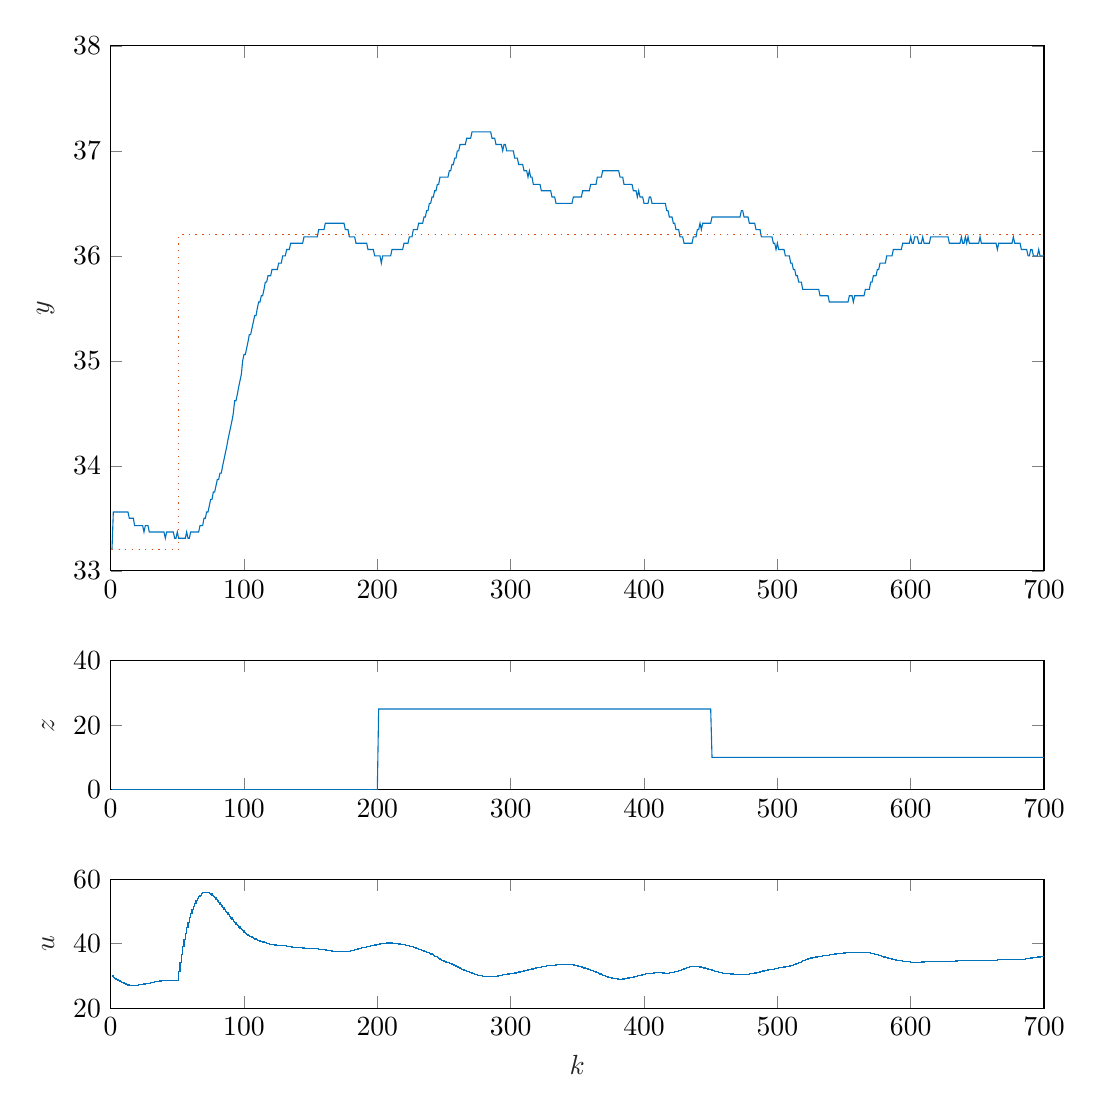
\begin{tikzpicture}

\begin{axis}[%
width=4.667in,
height=0.645in,
at={(0.583in,0.52in)},
scale only axis,
xmin=0,
xmax=700,
xtick={0,100,200,300,400,500,600,700},
xlabel style={font=\color{white!15!black}},
xlabel={$k$},
ymin=20,
ymax=60,
ytick={20,40,60},
ylabel style={font=\color{white!15!black}},
ylabel={$u$},
axis background/.style={fill=white}
]
\addplot[const plot, color=mycolor1, forget plot] table[row sep=crcr] {%
1	30\\
2	29.652\\
3	29.328\\
4	29.027\\
5	28.748\\
6	28.49\\
7	28.252\\
8	28.034\\
9	27.835\\
10	27.654\\
11	27.489\\
12	27.341\\
13	27.208\\
14	27.148\\
15	27.098\\
16	27.057\\
17	27.024\\
18	27.068\\
19	27.114\\
20	27.163\\
21	27.215\\
22	27.268\\
23	27.323\\
24	27.379\\
25	27.495\\
26	27.549\\
27	27.604\\
28	27.659\\
29	27.772\\
30	27.879\\
31	27.98\\
32	28.073\\
33	28.159\\
34	28.236\\
35	28.306\\
36	28.367\\
37	28.419\\
38	28.463\\
39	28.499\\
40	28.526\\
41	28.603\\
42	28.611\\
43	28.612\\
44	28.606\\
45	28.595\\
46	28.578\\
47	28.556\\
48	28.589\\
49	28.614\\
50	28.574\\
51	31.489\\
52	34.2\\
53	36.715\\
54	39.041\\
55	41.187\\
56	43.159\\
57	44.909\\
58	46.562\\
59	48.065\\
60	49.366\\
61	50.535\\
62	51.579\\
63	52.504\\
64	53.316\\
65	54.023\\
66	54.63\\
67	55.084\\
68	55.455\\
69	55.746\\
70	55.896\\
71	55.983\\
72	55.951\\
73	55.868\\
74	55.681\\
75	55.396\\
76	55.08\\
77	54.668\\
78	54.244\\
79	53.761\\
80	53.23\\
81	52.723\\
82	52.186\\
83	51.687\\
84	51.162\\
85	50.628\\
86	50.091\\
87	49.557\\
88	49.019\\
89	48.493\\
90	47.979\\
91	47.482\\
92	46.993\\
93	46.465\\
94	46.02\\
95	45.594\\
96	45.179\\
97	44.785\\
98	44.41\\
99	43.986\\
100	43.584\\
101	43.26\\
102	42.951\\
103	42.654\\
104	42.358\\
105	42.13\\
106	41.905\\
107	41.683\\
108	41.46\\
109	41.295\\
110	41.113\\
111	40.923\\
112	40.784\\
113	40.631\\
114	40.523\\
115	40.396\\
116	40.24\\
117	40.124\\
118	39.985\\
119	39.881\\
120	39.809\\
121	39.707\\
122	39.633\\
123	39.585\\
124	39.559\\
125	39.553\\
126	39.506\\
127	39.478\\
128	39.465\\
129	39.399\\
130	39.35\\
131	39.316\\
132	39.236\\
133	39.172\\
134	39.122\\
135	39.026\\
136	38.945\\
137	38.877\\
138	38.821\\
139	38.776\\
140	38.741\\
141	38.715\\
142	38.697\\
143	38.685\\
144	38.679\\
145	38.621\\
146	38.571\\
147	38.528\\
148	38.493\\
149	38.464\\
150	38.44\\
151	38.422\\
152	38.409\\
153	38.4\\
154	38.396\\
155	38.395\\
156	38.33\\
157	38.272\\
158	38.221\\
159	38.177\\
160	38.138\\
161	38.047\\
162	37.964\\
163	37.89\\
164	37.823\\
165	37.763\\
166	37.709\\
167	37.662\\
168	37.62\\
169	37.583\\
170	37.551\\
171	37.524\\
172	37.501\\
173	37.482\\
174	37.466\\
175	37.453\\
176	37.502\\
177	37.548\\
178	37.594\\
179	37.705\\
180	37.81\\
181	37.909\\
182	38.002\\
183	38.089\\
184	38.229\\
185	38.358\\
186	38.478\\
187	38.588\\
188	38.69\\
189	38.782\\
190	38.865\\
191	38.94\\
192	39.007\\
193	39.123\\
194	39.227\\
195	39.32\\
196	39.403\\
197	39.475\\
198	39.595\\
199	39.701\\
200	39.795\\
201	39.877\\
202	39.947\\
203	40.075\\
204	40.12\\
205	40.156\\
206	40.185\\
207	40.206\\
208	40.22\\
209	40.229\\
210	40.232\\
211	40.174\\
212	40.116\\
213	40.058\\
214	40.002\\
215	39.947\\
216	39.895\\
217	39.844\\
218	39.796\\
219	39.751\\
220	39.65\\
221	39.556\\
222	39.469\\
223	39.389\\
224	39.258\\
225	39.138\\
226	39.029\\
227	38.862\\
228	38.71\\
229	38.573\\
230	38.449\\
231	38.281\\
232	38.13\\
233	37.995\\
234	37.875\\
235	37.712\\
236	37.567\\
237	37.38\\
238	37.213\\
239	36.997\\
240	36.803\\
241	36.571\\
242	36.364\\
243	36.12\\
244	35.901\\
245	35.648\\
246	35.42\\
247	35.15\\
248	34.907\\
249	34.69\\
250	34.498\\
251	34.328\\
252	34.18\\
253	34.051\\
254	33.882\\
255	33.734\\
256	33.548\\
257	33.383\\
258	33.18\\
259	33\\
260	32.773\\
261	32.57\\
262	32.332\\
263	32.118\\
264	31.928\\
265	31.76\\
266	31.611\\
267	31.423\\
268	31.256\\
269	31.107\\
270	30.976\\
271	30.802\\
272	30.647\\
273	30.509\\
274	30.386\\
275	30.277\\
276	30.18\\
277	30.095\\
278	30.02\\
279	29.954\\
280	29.897\\
281	29.848\\
282	29.806\\
283	29.77\\
284	29.74\\
285	29.714\\
286	29.751\\
287	29.786\\
288	29.821\\
289	29.912\\
290	29.996\\
291	30.075\\
292	30.147\\
293	30.212\\
294	30.329\\
295	30.377\\
296	30.418\\
297	30.511\\
298	30.594\\
299	30.666\\
300	30.729\\
301	30.781\\
302	30.824\\
303	30.926\\
304	31.014\\
305	31.089\\
306	31.21\\
307	31.315\\
308	31.406\\
309	31.482\\
310	31.602\\
311	31.706\\
312	31.794\\
313	31.925\\
314	31.98\\
315	32.08\\
316	32.164\\
317	32.302\\
318	32.421\\
319	32.523\\
320	32.609\\
321	32.681\\
322	32.738\\
323	32.841\\
324	32.929\\
325	33.001\\
326	33.06\\
327	33.107\\
328	33.142\\
329	33.166\\
330	33.18\\
331	33.244\\
332	33.294\\
333	33.333\\
334	33.418\\
335	33.489\\
336	33.545\\
337	33.588\\
338	33.619\\
339	33.638\\
340	33.646\\
341	33.644\\
342	33.632\\
343	33.612\\
344	33.584\\
345	33.55\\
346	33.509\\
347	33.405\\
348	33.301\\
349	33.195\\
350	33.091\\
351	32.987\\
352	32.884\\
353	32.782\\
354	32.625\\
355	32.474\\
356	32.328\\
357	32.189\\
358	32.057\\
359	31.931\\
360	31.754\\
361	31.587\\
362	31.431\\
363	31.286\\
364	31.151\\
365	30.959\\
366	30.782\\
367	30.618\\
368	30.469\\
369	30.274\\
370	30.096\\
371	29.934\\
372	29.786\\
373	29.654\\
374	29.534\\
375	29.427\\
376	29.332\\
377	29.247\\
378	29.172\\
379	29.107\\
380	29.05\\
381	29\\
382	29.016\\
383	29.033\\
384	29.052\\
385	29.14\\
386	29.223\\
387	29.302\\
388	29.376\\
389	29.445\\
390	29.509\\
391	29.567\\
392	29.677\\
393	29.777\\
394	29.868\\
395	30.006\\
396	30.073\\
397	30.188\\
398	30.289\\
399	30.377\\
400	30.51\\
401	30.627\\
402	30.728\\
403	30.814\\
404	30.827\\
405	30.831\\
406	30.883\\
407	30.923\\
408	30.95\\
409	30.967\\
410	30.973\\
411	30.97\\
412	30.958\\
413	30.939\\
414	30.914\\
415	30.882\\
416	30.846\\
417	30.873\\
418	30.892\\
419	30.961\\
420	31.02\\
421	31.07\\
422	31.168\\
423	31.255\\
424	31.39\\
425	31.51\\
426	31.617\\
427	31.78\\
428	31.928\\
429	32.062\\
430	32.24\\
431	32.401\\
432	32.546\\
433	32.677\\
434	32.793\\
435	32.896\\
436	32.987\\
437	33.008\\
438	33.021\\
439	33.028\\
440	32.961\\
441	32.893\\
442	32.766\\
443	32.7\\
444	32.575\\
445	32.454\\
446	32.337\\
447	32.224\\
448	32.116\\
449	32.011\\
450	31.912\\
451	31.76\\
452	31.617\\
453	31.484\\
454	31.36\\
455	31.245\\
456	31.14\\
457	31.044\\
458	30.958\\
459	30.882\\
460	30.815\\
461	30.757\\
462	30.708\\
463	30.667\\
464	30.635\\
465	30.61\\
466	30.592\\
467	30.58\\
468	30.574\\
469	30.572\\
470	30.575\\
471	30.581\\
472	30.589\\
473	30.542\\
474	30.5\\
475	30.521\\
476	30.542\\
477	30.563\\
478	30.584\\
479	30.661\\
480	30.732\\
481	30.797\\
482	30.857\\
483	30.91\\
484	31.016\\
485	31.111\\
486	31.197\\
487	31.273\\
488	31.408\\
489	31.529\\
490	31.637\\
491	31.732\\
492	31.816\\
493	31.888\\
494	31.95\\
495	32.002\\
496	32.044\\
497	32.135\\
498	32.214\\
499	32.339\\
500	32.391\\
501	32.491\\
502	32.578\\
503	32.651\\
504	32.713\\
505	32.764\\
506	32.862\\
507	32.947\\
508	33.02\\
509	33.082\\
510	33.2\\
511	33.305\\
512	33.454\\
513	33.588\\
514	33.764\\
515	33.923\\
516	34.123\\
517	34.304\\
518	34.467\\
519	34.68\\
520	34.874\\
521	35.048\\
522	35.204\\
523	35.344\\
524	35.467\\
525	35.576\\
526	35.672\\
527	35.755\\
528	35.827\\
529	35.889\\
530	35.941\\
531	35.984\\
532	36.077\\
533	36.159\\
534	36.231\\
535	36.294\\
536	36.348\\
537	36.394\\
538	36.433\\
539	36.524\\
540	36.606\\
541	36.68\\
542	36.746\\
543	36.807\\
544	36.862\\
545	36.912\\
546	36.959\\
547	37.002\\
548	37.044\\
549	37.083\\
550	37.122\\
551	37.16\\
552	37.197\\
553	37.233\\
554	37.212\\
555	37.194\\
556	37.181\\
557	37.229\\
558	37.22\\
559	37.214\\
560	37.212\\
561	37.213\\
562	37.219\\
563	37.228\\
564	37.241\\
565	37.257\\
566	37.218\\
567	37.186\\
568	37.161\\
569	37.143\\
570	37.063\\
571	36.994\\
572	36.877\\
573	36.774\\
574	36.684\\
575	36.548\\
576	36.428\\
577	36.265\\
578	36.121\\
579	35.993\\
580	35.882\\
581	35.787\\
582	35.638\\
583	35.508\\
584	35.394\\
585	35.297\\
586	35.216\\
587	35.09\\
588	34.982\\
589	34.891\\
590	34.814\\
591	34.752\\
592	34.704\\
593	34.668\\
594	34.585\\
595	34.517\\
596	34.462\\
597	34.42\\
598	34.39\\
599	34.369\\
600	34.3\\
601	34.301\\
602	34.308\\
603	34.264\\
604	34.229\\
605	34.202\\
606	34.24\\
607	34.28\\
608	34.321\\
609	34.306\\
610	34.353\\
611	34.4\\
612	34.446\\
613	34.491\\
614	34.535\\
615	34.518\\
616	34.504\\
617	34.491\\
618	34.48\\
619	34.469\\
620	34.459\\
621	34.45\\
622	34.442\\
623	34.434\\
624	34.425\\
625	34.417\\
626	34.409\\
627	34.401\\
628	34.393\\
629	34.443\\
630	34.489\\
631	34.53\\
632	34.569\\
633	34.603\\
634	34.635\\
635	34.663\\
636	34.689\\
637	34.713\\
638	34.676\\
639	34.699\\
640	34.721\\
641	34.683\\
642	34.706\\
643	34.669\\
644	34.693\\
645	34.715\\
646	34.735\\
647	34.754\\
648	34.772\\
649	34.789\\
650	34.804\\
651	34.818\\
652	34.772\\
653	34.788\\
654	34.803\\
655	34.816\\
656	34.829\\
657	34.841\\
658	34.852\\
659	34.863\\
660	34.874\\
661	34.884\\
662	34.894\\
663	34.905\\
664	34.915\\
665	34.983\\
666	34.989\\
667	34.995\\
668	35.001\\
669	35.007\\
670	35.013\\
671	35.018\\
672	35.024\\
673	35.029\\
674	35.035\\
675	35.04\\
676	35.046\\
677	34.993\\
678	35.002\\
679	35.011\\
680	35.02\\
681	35.029\\
682	35.037\\
683	35.103\\
684	35.164\\
685	35.222\\
686	35.276\\
687	35.326\\
688	35.43\\
689	35.527\\
690	35.559\\
691	35.588\\
692	35.672\\
693	35.75\\
694	35.822\\
695	35.888\\
696	35.891\\
697	35.95\\
698	36.004\\
699	36.053\\
700	36.098\\
};
\end{axis}

\begin{axis}[%
width=4.667in,
height=0.645in,
at={(0.583in,1.613in)},
scale only axis,
xmin=0,
xmax=700,
xtick={0,100,200,300,400,500,600,700},
ymin=0,
ymax=40,
ytick={0,20,40},
ylabel style={font=\color{white!15!black}},
ylabel={$z$},
axis background/.style={fill=white}
]
\addplot [color=mycolor1, forget plot]
  table[row sep=crcr]{%
1	0\\
2	0\\
3	0\\
4	0\\
5	0\\
6	0\\
7	0\\
8	0\\
9	0\\
10	0\\
11	0\\
12	0\\
13	0\\
14	0\\
15	0\\
16	0\\
17	0\\
18	0\\
19	0\\
20	0\\
21	0\\
22	0\\
23	0\\
24	0\\
25	0\\
26	0\\
27	0\\
28	0\\
29	0\\
30	0\\
31	0\\
32	0\\
33	0\\
34	0\\
35	0\\
36	0\\
37	0\\
38	0\\
39	0\\
40	0\\
41	0\\
42	0\\
43	0\\
44	0\\
45	0\\
46	0\\
47	0\\
48	0\\
49	0\\
50	0\\
51	0\\
52	0\\
53	0\\
54	0\\
55	0\\
56	0\\
57	0\\
58	0\\
59	0\\
60	0\\
61	0\\
62	0\\
63	0\\
64	0\\
65	0\\
66	0\\
67	0\\
68	0\\
69	0\\
70	0\\
71	0\\
72	0\\
73	0\\
74	0\\
75	0\\
76	0\\
77	0\\
78	0\\
79	0\\
80	0\\
81	0\\
82	0\\
83	0\\
84	0\\
85	0\\
86	0\\
87	0\\
88	0\\
89	0\\
90	0\\
91	0\\
92	0\\
93	0\\
94	0\\
95	0\\
96	0\\
97	0\\
98	0\\
99	0\\
100	0\\
101	0\\
102	0\\
103	0\\
104	0\\
105	0\\
106	0\\
107	0\\
108	0\\
109	0\\
110	0\\
111	0\\
112	0\\
113	0\\
114	0\\
115	0\\
116	0\\
117	0\\
118	0\\
119	0\\
120	0\\
121	0\\
122	0\\
123	0\\
124	0\\
125	0\\
126	0\\
127	0\\
128	0\\
129	0\\
130	0\\
131	0\\
132	0\\
133	0\\
134	0\\
135	0\\
136	0\\
137	0\\
138	0\\
139	0\\
140	0\\
141	0\\
142	0\\
143	0\\
144	0\\
145	0\\
146	0\\
147	0\\
148	0\\
149	0\\
150	0\\
151	0\\
152	0\\
153	0\\
154	0\\
155	0\\
156	0\\
157	0\\
158	0\\
159	0\\
160	0\\
161	0\\
162	0\\
163	0\\
164	0\\
165	0\\
166	0\\
167	0\\
168	0\\
169	0\\
170	0\\
171	0\\
172	0\\
173	0\\
174	0\\
175	0\\
176	0\\
177	0\\
178	0\\
179	0\\
180	0\\
181	0\\
182	0\\
183	0\\
184	0\\
185	0\\
186	0\\
187	0\\
188	0\\
189	0\\
190	0\\
191	0\\
192	0\\
193	0\\
194	0\\
195	0\\
196	0\\
197	0\\
198	0\\
199	0\\
200	0\\
201	25\\
202	25\\
203	25\\
204	25\\
205	25\\
206	25\\
207	25\\
208	25\\
209	25\\
210	25\\
211	25\\
212	25\\
213	25\\
214	25\\
215	25\\
216	25\\
217	25\\
218	25\\
219	25\\
220	25\\
221	25\\
222	25\\
223	25\\
224	25\\
225	25\\
226	25\\
227	25\\
228	25\\
229	25\\
230	25\\
231	25\\
232	25\\
233	25\\
234	25\\
235	25\\
236	25\\
237	25\\
238	25\\
239	25\\
240	25\\
241	25\\
242	25\\
243	25\\
244	25\\
245	25\\
246	25\\
247	25\\
248	25\\
249	25\\
250	25\\
251	25\\
252	25\\
253	25\\
254	25\\
255	25\\
256	25\\
257	25\\
258	25\\
259	25\\
260	25\\
261	25\\
262	25\\
263	25\\
264	25\\
265	25\\
266	25\\
267	25\\
268	25\\
269	25\\
270	25\\
271	25\\
272	25\\
273	25\\
274	25\\
275	25\\
276	25\\
277	25\\
278	25\\
279	25\\
280	25\\
281	25\\
282	25\\
283	25\\
284	25\\
285	25\\
286	25\\
287	25\\
288	25\\
289	25\\
290	25\\
291	25\\
292	25\\
293	25\\
294	25\\
295	25\\
296	25\\
297	25\\
298	25\\
299	25\\
300	25\\
301	25\\
302	25\\
303	25\\
304	25\\
305	25\\
306	25\\
307	25\\
308	25\\
309	25\\
310	25\\
311	25\\
312	25\\
313	25\\
314	25\\
315	25\\
316	25\\
317	25\\
318	25\\
319	25\\
320	25\\
321	25\\
322	25\\
323	25\\
324	25\\
325	25\\
326	25\\
327	25\\
328	25\\
329	25\\
330	25\\
331	25\\
332	25\\
333	25\\
334	25\\
335	25\\
336	25\\
337	25\\
338	25\\
339	25\\
340	25\\
341	25\\
342	25\\
343	25\\
344	25\\
345	25\\
346	25\\
347	25\\
348	25\\
349	25\\
350	25\\
351	25\\
352	25\\
353	25\\
354	25\\
355	25\\
356	25\\
357	25\\
358	25\\
359	25\\
360	25\\
361	25\\
362	25\\
363	25\\
364	25\\
365	25\\
366	25\\
367	25\\
368	25\\
369	25\\
370	25\\
371	25\\
372	25\\
373	25\\
374	25\\
375	25\\
376	25\\
377	25\\
378	25\\
379	25\\
380	25\\
381	25\\
382	25\\
383	25\\
384	25\\
385	25\\
386	25\\
387	25\\
388	25\\
389	25\\
390	25\\
391	25\\
392	25\\
393	25\\
394	25\\
395	25\\
396	25\\
397	25\\
398	25\\
399	25\\
400	25\\
401	25\\
402	25\\
403	25\\
404	25\\
405	25\\
406	25\\
407	25\\
408	25\\
409	25\\
410	25\\
411	25\\
412	25\\
413	25\\
414	25\\
415	25\\
416	25\\
417	25\\
418	25\\
419	25\\
420	25\\
421	25\\
422	25\\
423	25\\
424	25\\
425	25\\
426	25\\
427	25\\
428	25\\
429	25\\
430	25\\
431	25\\
432	25\\
433	25\\
434	25\\
435	25\\
436	25\\
437	25\\
438	25\\
439	25\\
440	25\\
441	25\\
442	25\\
443	25\\
444	25\\
445	25\\
446	25\\
447	25\\
448	25\\
449	25\\
450	25\\
451	10\\
452	10\\
453	10\\
454	10\\
455	10\\
456	10\\
457	10\\
458	10\\
459	10\\
460	10\\
461	10\\
462	10\\
463	10\\
464	10\\
465	10\\
466	10\\
467	10\\
468	10\\
469	10\\
470	10\\
471	10\\
472	10\\
473	10\\
474	10\\
475	10\\
476	10\\
477	10\\
478	10\\
479	10\\
480	10\\
481	10\\
482	10\\
483	10\\
484	10\\
485	10\\
486	10\\
487	10\\
488	10\\
489	10\\
490	10\\
491	10\\
492	10\\
493	10\\
494	10\\
495	10\\
496	10\\
497	10\\
498	10\\
499	10\\
500	10\\
501	10\\
502	10\\
503	10\\
504	10\\
505	10\\
506	10\\
507	10\\
508	10\\
509	10\\
510	10\\
511	10\\
512	10\\
513	10\\
514	10\\
515	10\\
516	10\\
517	10\\
518	10\\
519	10\\
520	10\\
521	10\\
522	10\\
523	10\\
524	10\\
525	10\\
526	10\\
527	10\\
528	10\\
529	10\\
530	10\\
531	10\\
532	10\\
533	10\\
534	10\\
535	10\\
536	10\\
537	10\\
538	10\\
539	10\\
540	10\\
541	10\\
542	10\\
543	10\\
544	10\\
545	10\\
546	10\\
547	10\\
548	10\\
549	10\\
550	10\\
551	10\\
552	10\\
553	10\\
554	10\\
555	10\\
556	10\\
557	10\\
558	10\\
559	10\\
560	10\\
561	10\\
562	10\\
563	10\\
564	10\\
565	10\\
566	10\\
567	10\\
568	10\\
569	10\\
570	10\\
571	10\\
572	10\\
573	10\\
574	10\\
575	10\\
576	10\\
577	10\\
578	10\\
579	10\\
580	10\\
581	10\\
582	10\\
583	10\\
584	10\\
585	10\\
586	10\\
587	10\\
588	10\\
589	10\\
590	10\\
591	10\\
592	10\\
593	10\\
594	10\\
595	10\\
596	10\\
597	10\\
598	10\\
599	10\\
600	10\\
601	10\\
602	10\\
603	10\\
604	10\\
605	10\\
606	10\\
607	10\\
608	10\\
609	10\\
610	10\\
611	10\\
612	10\\
613	10\\
614	10\\
615	10\\
616	10\\
617	10\\
618	10\\
619	10\\
620	10\\
621	10\\
622	10\\
623	10\\
624	10\\
625	10\\
626	10\\
627	10\\
628	10\\
629	10\\
630	10\\
631	10\\
632	10\\
633	10\\
634	10\\
635	10\\
636	10\\
637	10\\
638	10\\
639	10\\
640	10\\
641	10\\
642	10\\
643	10\\
644	10\\
645	10\\
646	10\\
647	10\\
648	10\\
649	10\\
650	10\\
651	10\\
652	10\\
653	10\\
654	10\\
655	10\\
656	10\\
657	10\\
658	10\\
659	10\\
660	10\\
661	10\\
662	10\\
663	10\\
664	10\\
665	10\\
666	10\\
667	10\\
668	10\\
669	10\\
670	10\\
671	10\\
672	10\\
673	10\\
674	10\\
675	10\\
676	10\\
677	10\\
678	10\\
679	10\\
680	10\\
681	10\\
682	10\\
683	10\\
684	10\\
685	10\\
686	10\\
687	10\\
688	10\\
689	10\\
690	10\\
691	10\\
692	10\\
693	10\\
694	10\\
695	10\\
696	10\\
697	10\\
698	10\\
699	10\\
700	10\\
};
\end{axis}

\begin{axis}[%
width=4.667in,
height=2.625in,
at={(0.583in,2.707in)},
scale only axis,
xmin=0,
xmax=700,
xtick={0,100,200,300,400,500,600,700},
ymin=33,
ymax=38,
ytick={33,34,35,36,37,38},
ylabel style={font=\color{white!15!black}},
ylabel={$y$},
axis background/.style={fill=white}
]
\addplot [color=mycolor1, forget plot]
  table[row sep=crcr]{%
1	33.2\\
2	33.56\\
3	33.56\\
4	33.56\\
5	33.56\\
6	33.56\\
7	33.56\\
8	33.56\\
9	33.56\\
10	33.56\\
11	33.56\\
12	33.56\\
13	33.56\\
14	33.5\\
15	33.5\\
16	33.5\\
17	33.5\\
18	33.43\\
19	33.43\\
20	33.43\\
21	33.43\\
22	33.43\\
23	33.43\\
24	33.43\\
25	33.37\\
26	33.43\\
27	33.43\\
28	33.43\\
29	33.37\\
30	33.37\\
31	33.37\\
32	33.37\\
33	33.37\\
34	33.37\\
35	33.37\\
36	33.37\\
37	33.37\\
38	33.37\\
39	33.37\\
40	33.37\\
41	33.31\\
42	33.37\\
43	33.37\\
44	33.37\\
45	33.37\\
46	33.37\\
47	33.37\\
48	33.31\\
49	33.31\\
50	33.37\\
51	33.31\\
52	33.31\\
53	33.31\\
54	33.31\\
55	33.31\\
56	33.31\\
57	33.37\\
58	33.31\\
59	33.31\\
60	33.37\\
61	33.37\\
62	33.37\\
63	33.37\\
64	33.37\\
65	33.37\\
66	33.37\\
67	33.43\\
68	33.43\\
69	33.43\\
70	33.5\\
71	33.5\\
72	33.56\\
73	33.56\\
74	33.62\\
75	33.68\\
76	33.68\\
77	33.75\\
78	33.75\\
79	33.81\\
80	33.87\\
81	33.87\\
82	33.93\\
83	33.93\\
84	34\\
85	34.06\\
86	34.12\\
87	34.18\\
88	34.25\\
89	34.31\\
90	34.37\\
91	34.43\\
92	34.5\\
93	34.62\\
94	34.62\\
95	34.68\\
96	34.75\\
97	34.81\\
98	34.87\\
99	35\\
100	35.06\\
101	35.06\\
102	35.12\\
103	35.18\\
104	35.25\\
105	35.25\\
106	35.31\\
107	35.37\\
108	35.43\\
109	35.43\\
110	35.5\\
111	35.56\\
112	35.56\\
113	35.62\\
114	35.62\\
115	35.68\\
116	35.75\\
117	35.75\\
118	35.81\\
119	35.81\\
120	35.81\\
121	35.87\\
122	35.87\\
123	35.87\\
124	35.87\\
125	35.87\\
126	35.93\\
127	35.93\\
128	35.93\\
129	36\\
130	36\\
131	36\\
132	36.06\\
133	36.06\\
134	36.06\\
135	36.12\\
136	36.12\\
137	36.12\\
138	36.12\\
139	36.12\\
140	36.12\\
141	36.12\\
142	36.12\\
143	36.12\\
144	36.12\\
145	36.18\\
146	36.18\\
147	36.18\\
148	36.18\\
149	36.18\\
150	36.18\\
151	36.18\\
152	36.18\\
153	36.18\\
154	36.18\\
155	36.18\\
156	36.25\\
157	36.25\\
158	36.25\\
159	36.25\\
160	36.25\\
161	36.31\\
162	36.31\\
163	36.31\\
164	36.31\\
165	36.31\\
166	36.31\\
167	36.31\\
168	36.31\\
169	36.31\\
170	36.31\\
171	36.31\\
172	36.31\\
173	36.31\\
174	36.31\\
175	36.31\\
176	36.25\\
177	36.25\\
178	36.25\\
179	36.18\\
180	36.18\\
181	36.18\\
182	36.18\\
183	36.18\\
184	36.12\\
185	36.12\\
186	36.12\\
187	36.12\\
188	36.12\\
189	36.12\\
190	36.12\\
191	36.12\\
192	36.12\\
193	36.06\\
194	36.06\\
195	36.06\\
196	36.06\\
197	36.06\\
198	36\\
199	36\\
200	36\\
201	36\\
202	36\\
203	35.93\\
204	36\\
205	36\\
206	36\\
207	36\\
208	36\\
209	36\\
210	36\\
211	36.06\\
212	36.06\\
213	36.06\\
214	36.06\\
215	36.06\\
216	36.06\\
217	36.06\\
218	36.06\\
219	36.06\\
220	36.12\\
221	36.12\\
222	36.12\\
223	36.12\\
224	36.18\\
225	36.18\\
226	36.18\\
227	36.25\\
228	36.25\\
229	36.25\\
230	36.25\\
231	36.31\\
232	36.31\\
233	36.31\\
234	36.31\\
235	36.37\\
236	36.37\\
237	36.43\\
238	36.43\\
239	36.5\\
240	36.5\\
241	36.56\\
242	36.56\\
243	36.62\\
244	36.62\\
245	36.68\\
246	36.68\\
247	36.75\\
248	36.75\\
249	36.75\\
250	36.75\\
251	36.75\\
252	36.75\\
253	36.75\\
254	36.81\\
255	36.81\\
256	36.87\\
257	36.87\\
258	36.93\\
259	36.93\\
260	37\\
261	37\\
262	37.06\\
263	37.06\\
264	37.06\\
265	37.06\\
266	37.06\\
267	37.12\\
268	37.12\\
269	37.12\\
270	37.12\\
271	37.18\\
272	37.18\\
273	37.18\\
274	37.18\\
275	37.18\\
276	37.18\\
277	37.18\\
278	37.18\\
279	37.18\\
280	37.18\\
281	37.18\\
282	37.18\\
283	37.18\\
284	37.18\\
285	37.18\\
286	37.12\\
287	37.12\\
288	37.12\\
289	37.06\\
290	37.06\\
291	37.06\\
292	37.06\\
293	37.06\\
294	37\\
295	37.06\\
296	37.06\\
297	37\\
298	37\\
299	37\\
300	37\\
301	37\\
302	37\\
303	36.93\\
304	36.93\\
305	36.93\\
306	36.87\\
307	36.87\\
308	36.87\\
309	36.87\\
310	36.81\\
311	36.81\\
312	36.81\\
313	36.75\\
314	36.81\\
315	36.75\\
316	36.75\\
317	36.68\\
318	36.68\\
319	36.68\\
320	36.68\\
321	36.68\\
322	36.68\\
323	36.62\\
324	36.62\\
325	36.62\\
326	36.62\\
327	36.62\\
328	36.62\\
329	36.62\\
330	36.62\\
331	36.56\\
332	36.56\\
333	36.56\\
334	36.5\\
335	36.5\\
336	36.5\\
337	36.5\\
338	36.5\\
339	36.5\\
340	36.5\\
341	36.5\\
342	36.5\\
343	36.5\\
344	36.5\\
345	36.5\\
346	36.5\\
347	36.56\\
348	36.56\\
349	36.56\\
350	36.56\\
351	36.56\\
352	36.56\\
353	36.56\\
354	36.62\\
355	36.62\\
356	36.62\\
357	36.62\\
358	36.62\\
359	36.62\\
360	36.68\\
361	36.68\\
362	36.68\\
363	36.68\\
364	36.68\\
365	36.75\\
366	36.75\\
367	36.75\\
368	36.75\\
369	36.81\\
370	36.81\\
371	36.81\\
372	36.81\\
373	36.81\\
374	36.81\\
375	36.81\\
376	36.81\\
377	36.81\\
378	36.81\\
379	36.81\\
380	36.81\\
381	36.81\\
382	36.75\\
383	36.75\\
384	36.75\\
385	36.68\\
386	36.68\\
387	36.68\\
388	36.68\\
389	36.68\\
390	36.68\\
391	36.68\\
392	36.62\\
393	36.62\\
394	36.62\\
395	36.56\\
396	36.62\\
397	36.56\\
398	36.56\\
399	36.56\\
400	36.5\\
401	36.5\\
402	36.5\\
403	36.5\\
404	36.56\\
405	36.56\\
406	36.5\\
407	36.5\\
408	36.5\\
409	36.5\\
410	36.5\\
411	36.5\\
412	36.5\\
413	36.5\\
414	36.5\\
415	36.5\\
416	36.5\\
417	36.43\\
418	36.43\\
419	36.37\\
420	36.37\\
421	36.37\\
422	36.31\\
423	36.31\\
424	36.25\\
425	36.25\\
426	36.25\\
427	36.18\\
428	36.18\\
429	36.18\\
430	36.12\\
431	36.12\\
432	36.12\\
433	36.12\\
434	36.12\\
435	36.12\\
436	36.12\\
437	36.18\\
438	36.18\\
439	36.18\\
440	36.25\\
441	36.25\\
442	36.31\\
443	36.25\\
444	36.31\\
445	36.31\\
446	36.31\\
447	36.31\\
448	36.31\\
449	36.31\\
450	36.31\\
451	36.37\\
452	36.37\\
453	36.37\\
454	36.37\\
455	36.37\\
456	36.37\\
457	36.37\\
458	36.37\\
459	36.37\\
460	36.37\\
461	36.37\\
462	36.37\\
463	36.37\\
464	36.37\\
465	36.37\\
466	36.37\\
467	36.37\\
468	36.37\\
469	36.37\\
470	36.37\\
471	36.37\\
472	36.37\\
473	36.43\\
474	36.43\\
475	36.37\\
476	36.37\\
477	36.37\\
478	36.37\\
479	36.31\\
480	36.31\\
481	36.31\\
482	36.31\\
483	36.31\\
484	36.25\\
485	36.25\\
486	36.25\\
487	36.25\\
488	36.18\\
489	36.18\\
490	36.18\\
491	36.18\\
492	36.18\\
493	36.18\\
494	36.18\\
495	36.18\\
496	36.18\\
497	36.12\\
498	36.12\\
499	36.06\\
500	36.12\\
501	36.06\\
502	36.06\\
503	36.06\\
504	36.06\\
505	36.06\\
506	36\\
507	36\\
508	36\\
509	36\\
510	35.93\\
511	35.93\\
512	35.87\\
513	35.87\\
514	35.81\\
515	35.81\\
516	35.75\\
517	35.75\\
518	35.75\\
519	35.68\\
520	35.68\\
521	35.68\\
522	35.68\\
523	35.68\\
524	35.68\\
525	35.68\\
526	35.68\\
527	35.68\\
528	35.68\\
529	35.68\\
530	35.68\\
531	35.68\\
532	35.62\\
533	35.62\\
534	35.62\\
535	35.62\\
536	35.62\\
537	35.62\\
538	35.62\\
539	35.56\\
540	35.56\\
541	35.56\\
542	35.56\\
543	35.56\\
544	35.56\\
545	35.56\\
546	35.56\\
547	35.56\\
548	35.56\\
549	35.56\\
550	35.56\\
551	35.56\\
552	35.56\\
553	35.56\\
554	35.62\\
555	35.62\\
556	35.62\\
557	35.56\\
558	35.62\\
559	35.62\\
560	35.62\\
561	35.62\\
562	35.62\\
563	35.62\\
564	35.62\\
565	35.62\\
566	35.68\\
567	35.68\\
568	35.68\\
569	35.68\\
570	35.75\\
571	35.75\\
572	35.81\\
573	35.81\\
574	35.81\\
575	35.87\\
576	35.87\\
577	35.93\\
578	35.93\\
579	35.93\\
580	35.93\\
581	35.93\\
582	36\\
583	36\\
584	36\\
585	36\\
586	36\\
587	36.06\\
588	36.06\\
589	36.06\\
590	36.06\\
591	36.06\\
592	36.06\\
593	36.06\\
594	36.12\\
595	36.12\\
596	36.12\\
597	36.12\\
598	36.12\\
599	36.12\\
600	36.18\\
601	36.12\\
602	36.12\\
603	36.18\\
604	36.18\\
605	36.18\\
606	36.12\\
607	36.12\\
608	36.12\\
609	36.18\\
610	36.12\\
611	36.12\\
612	36.12\\
613	36.12\\
614	36.12\\
615	36.18\\
616	36.18\\
617	36.18\\
618	36.18\\
619	36.18\\
620	36.18\\
621	36.18\\
622	36.18\\
623	36.18\\
624	36.18\\
625	36.18\\
626	36.18\\
627	36.18\\
628	36.18\\
629	36.12\\
630	36.12\\
631	36.12\\
632	36.12\\
633	36.12\\
634	36.12\\
635	36.12\\
636	36.12\\
637	36.12\\
638	36.18\\
639	36.12\\
640	36.12\\
641	36.18\\
642	36.12\\
643	36.18\\
644	36.12\\
645	36.12\\
646	36.12\\
647	36.12\\
648	36.12\\
649	36.12\\
650	36.12\\
651	36.12\\
652	36.18\\
653	36.12\\
654	36.12\\
655	36.12\\
656	36.12\\
657	36.12\\
658	36.12\\
659	36.12\\
660	36.12\\
661	36.12\\
662	36.12\\
663	36.12\\
664	36.12\\
665	36.06\\
666	36.12\\
667	36.12\\
668	36.12\\
669	36.12\\
670	36.12\\
671	36.12\\
672	36.12\\
673	36.12\\
674	36.12\\
675	36.12\\
676	36.12\\
677	36.18\\
678	36.12\\
679	36.12\\
680	36.12\\
681	36.12\\
682	36.12\\
683	36.06\\
684	36.06\\
685	36.06\\
686	36.06\\
687	36.06\\
688	36\\
689	36\\
690	36.06\\
691	36.06\\
692	36\\
693	36\\
694	36\\
695	36\\
696	36.06\\
697	36\\
698	36\\
699	36\\
700	36\\
};
\addplot[const plot, color=mycolor2, dotted, forget plot] table[row sep=crcr] {%
1	33.2\\
2	33.2\\
3	33.2\\
4	33.2\\
5	33.2\\
6	33.2\\
7	33.2\\
8	33.2\\
9	33.2\\
10	33.2\\
11	33.2\\
12	33.2\\
13	33.2\\
14	33.2\\
15	33.2\\
16	33.2\\
17	33.2\\
18	33.2\\
19	33.2\\
20	33.2\\
21	33.2\\
22	33.2\\
23	33.2\\
24	33.2\\
25	33.2\\
26	33.2\\
27	33.2\\
28	33.2\\
29	33.2\\
30	33.2\\
31	33.2\\
32	33.2\\
33	33.2\\
34	33.2\\
35	33.2\\
36	33.2\\
37	33.2\\
38	33.2\\
39	33.2\\
40	33.2\\
41	33.2\\
42	33.2\\
43	33.2\\
44	33.2\\
45	33.2\\
46	33.2\\
47	33.2\\
48	33.2\\
49	33.2\\
50	33.2\\
51	36.2\\
52	36.2\\
53	36.2\\
54	36.2\\
55	36.2\\
56	36.2\\
57	36.2\\
58	36.2\\
59	36.2\\
60	36.2\\
61	36.2\\
62	36.2\\
63	36.2\\
64	36.2\\
65	36.2\\
66	36.2\\
67	36.2\\
68	36.2\\
69	36.2\\
70	36.2\\
71	36.2\\
72	36.2\\
73	36.2\\
74	36.2\\
75	36.2\\
76	36.2\\
77	36.2\\
78	36.2\\
79	36.2\\
80	36.2\\
81	36.2\\
82	36.2\\
83	36.2\\
84	36.2\\
85	36.2\\
86	36.2\\
87	36.2\\
88	36.2\\
89	36.2\\
90	36.2\\
91	36.2\\
92	36.2\\
93	36.2\\
94	36.2\\
95	36.2\\
96	36.2\\
97	36.2\\
98	36.2\\
99	36.2\\
100	36.2\\
101	36.2\\
102	36.2\\
103	36.2\\
104	36.2\\
105	36.2\\
106	36.2\\
107	36.2\\
108	36.2\\
109	36.2\\
110	36.2\\
111	36.2\\
112	36.2\\
113	36.2\\
114	36.2\\
115	36.2\\
116	36.2\\
117	36.2\\
118	36.2\\
119	36.2\\
120	36.2\\
121	36.2\\
122	36.2\\
123	36.2\\
124	36.2\\
125	36.2\\
126	36.2\\
127	36.2\\
128	36.2\\
129	36.2\\
130	36.2\\
131	36.2\\
132	36.2\\
133	36.2\\
134	36.2\\
135	36.2\\
136	36.2\\
137	36.2\\
138	36.2\\
139	36.2\\
140	36.2\\
141	36.2\\
142	36.2\\
143	36.2\\
144	36.2\\
145	36.2\\
146	36.2\\
147	36.2\\
148	36.2\\
149	36.2\\
150	36.2\\
151	36.2\\
152	36.2\\
153	36.2\\
154	36.2\\
155	36.2\\
156	36.2\\
157	36.2\\
158	36.2\\
159	36.2\\
160	36.2\\
161	36.2\\
162	36.2\\
163	36.2\\
164	36.2\\
165	36.2\\
166	36.2\\
167	36.2\\
168	36.2\\
169	36.2\\
170	36.2\\
171	36.2\\
172	36.2\\
173	36.2\\
174	36.2\\
175	36.2\\
176	36.2\\
177	36.2\\
178	36.2\\
179	36.2\\
180	36.2\\
181	36.2\\
182	36.2\\
183	36.2\\
184	36.2\\
185	36.2\\
186	36.2\\
187	36.2\\
188	36.2\\
189	36.2\\
190	36.2\\
191	36.2\\
192	36.2\\
193	36.2\\
194	36.2\\
195	36.2\\
196	36.2\\
197	36.2\\
198	36.2\\
199	36.2\\
200	36.2\\
201	36.2\\
202	36.2\\
203	36.2\\
204	36.2\\
205	36.2\\
206	36.2\\
207	36.2\\
208	36.2\\
209	36.2\\
210	36.2\\
211	36.2\\
212	36.2\\
213	36.2\\
214	36.2\\
215	36.2\\
216	36.2\\
217	36.2\\
218	36.2\\
219	36.2\\
220	36.2\\
221	36.2\\
222	36.2\\
223	36.2\\
224	36.2\\
225	36.2\\
226	36.2\\
227	36.2\\
228	36.2\\
229	36.2\\
230	36.2\\
231	36.2\\
232	36.2\\
233	36.2\\
234	36.2\\
235	36.2\\
236	36.2\\
237	36.2\\
238	36.2\\
239	36.2\\
240	36.2\\
241	36.2\\
242	36.2\\
243	36.2\\
244	36.2\\
245	36.2\\
246	36.2\\
247	36.2\\
248	36.2\\
249	36.2\\
250	36.2\\
251	36.2\\
252	36.2\\
253	36.2\\
254	36.2\\
255	36.2\\
256	36.2\\
257	36.2\\
258	36.2\\
259	36.2\\
260	36.2\\
261	36.2\\
262	36.2\\
263	36.2\\
264	36.2\\
265	36.2\\
266	36.2\\
267	36.2\\
268	36.2\\
269	36.2\\
270	36.2\\
271	36.2\\
272	36.2\\
273	36.2\\
274	36.2\\
275	36.2\\
276	36.2\\
277	36.2\\
278	36.2\\
279	36.2\\
280	36.2\\
281	36.2\\
282	36.2\\
283	36.2\\
284	36.2\\
285	36.2\\
286	36.2\\
287	36.2\\
288	36.2\\
289	36.2\\
290	36.2\\
291	36.2\\
292	36.2\\
293	36.2\\
294	36.2\\
295	36.2\\
296	36.2\\
297	36.2\\
298	36.2\\
299	36.2\\
300	36.2\\
301	36.2\\
302	36.2\\
303	36.2\\
304	36.2\\
305	36.2\\
306	36.2\\
307	36.2\\
308	36.2\\
309	36.2\\
310	36.2\\
311	36.2\\
312	36.2\\
313	36.2\\
314	36.2\\
315	36.2\\
316	36.2\\
317	36.2\\
318	36.2\\
319	36.2\\
320	36.2\\
321	36.2\\
322	36.2\\
323	36.2\\
324	36.2\\
325	36.2\\
326	36.2\\
327	36.2\\
328	36.2\\
329	36.2\\
330	36.2\\
331	36.2\\
332	36.2\\
333	36.2\\
334	36.2\\
335	36.2\\
336	36.2\\
337	36.2\\
338	36.2\\
339	36.2\\
340	36.2\\
341	36.2\\
342	36.2\\
343	36.2\\
344	36.2\\
345	36.2\\
346	36.2\\
347	36.2\\
348	36.2\\
349	36.2\\
350	36.2\\
351	36.2\\
352	36.2\\
353	36.2\\
354	36.2\\
355	36.2\\
356	36.2\\
357	36.2\\
358	36.2\\
359	36.2\\
360	36.2\\
361	36.2\\
362	36.2\\
363	36.2\\
364	36.2\\
365	36.2\\
366	36.2\\
367	36.2\\
368	36.2\\
369	36.2\\
370	36.2\\
371	36.2\\
372	36.2\\
373	36.2\\
374	36.2\\
375	36.2\\
376	36.2\\
377	36.2\\
378	36.2\\
379	36.2\\
380	36.2\\
381	36.2\\
382	36.2\\
383	36.2\\
384	36.2\\
385	36.2\\
386	36.2\\
387	36.2\\
388	36.2\\
389	36.2\\
390	36.2\\
391	36.2\\
392	36.2\\
393	36.2\\
394	36.2\\
395	36.2\\
396	36.2\\
397	36.2\\
398	36.2\\
399	36.2\\
400	36.2\\
401	36.2\\
402	36.2\\
403	36.2\\
404	36.2\\
405	36.2\\
406	36.2\\
407	36.2\\
408	36.2\\
409	36.2\\
410	36.2\\
411	36.2\\
412	36.2\\
413	36.2\\
414	36.2\\
415	36.2\\
416	36.2\\
417	36.2\\
418	36.2\\
419	36.2\\
420	36.2\\
421	36.2\\
422	36.2\\
423	36.2\\
424	36.2\\
425	36.2\\
426	36.2\\
427	36.2\\
428	36.2\\
429	36.2\\
430	36.2\\
431	36.2\\
432	36.2\\
433	36.2\\
434	36.2\\
435	36.2\\
436	36.2\\
437	36.2\\
438	36.2\\
439	36.2\\
440	36.2\\
441	36.2\\
442	36.2\\
443	36.2\\
444	36.2\\
445	36.2\\
446	36.2\\
447	36.2\\
448	36.2\\
449	36.2\\
450	36.2\\
451	36.2\\
452	36.2\\
453	36.2\\
454	36.2\\
455	36.2\\
456	36.2\\
457	36.2\\
458	36.2\\
459	36.2\\
460	36.2\\
461	36.2\\
462	36.2\\
463	36.2\\
464	36.2\\
465	36.2\\
466	36.2\\
467	36.2\\
468	36.2\\
469	36.2\\
470	36.2\\
471	36.2\\
472	36.2\\
473	36.2\\
474	36.2\\
475	36.2\\
476	36.2\\
477	36.2\\
478	36.2\\
479	36.2\\
480	36.2\\
481	36.2\\
482	36.2\\
483	36.2\\
484	36.2\\
485	36.2\\
486	36.2\\
487	36.2\\
488	36.2\\
489	36.2\\
490	36.2\\
491	36.2\\
492	36.2\\
493	36.2\\
494	36.2\\
495	36.2\\
496	36.2\\
497	36.2\\
498	36.2\\
499	36.2\\
500	36.2\\
501	36.2\\
502	36.2\\
503	36.2\\
504	36.2\\
505	36.2\\
506	36.2\\
507	36.2\\
508	36.2\\
509	36.2\\
510	36.2\\
511	36.2\\
512	36.2\\
513	36.2\\
514	36.2\\
515	36.2\\
516	36.2\\
517	36.2\\
518	36.2\\
519	36.2\\
520	36.2\\
521	36.2\\
522	36.2\\
523	36.2\\
524	36.2\\
525	36.2\\
526	36.2\\
527	36.2\\
528	36.2\\
529	36.2\\
530	36.2\\
531	36.2\\
532	36.2\\
533	36.2\\
534	36.2\\
535	36.2\\
536	36.2\\
537	36.2\\
538	36.2\\
539	36.2\\
540	36.2\\
541	36.2\\
542	36.2\\
543	36.2\\
544	36.2\\
545	36.2\\
546	36.2\\
547	36.2\\
548	36.2\\
549	36.2\\
550	36.2\\
551	36.2\\
552	36.2\\
553	36.2\\
554	36.2\\
555	36.2\\
556	36.2\\
557	36.2\\
558	36.2\\
559	36.2\\
560	36.2\\
561	36.2\\
562	36.2\\
563	36.2\\
564	36.2\\
565	36.2\\
566	36.2\\
567	36.2\\
568	36.2\\
569	36.2\\
570	36.2\\
571	36.2\\
572	36.2\\
573	36.2\\
574	36.2\\
575	36.2\\
576	36.2\\
577	36.2\\
578	36.2\\
579	36.2\\
580	36.2\\
581	36.2\\
582	36.2\\
583	36.2\\
584	36.2\\
585	36.2\\
586	36.2\\
587	36.2\\
588	36.2\\
589	36.2\\
590	36.2\\
591	36.2\\
592	36.2\\
593	36.2\\
594	36.2\\
595	36.2\\
596	36.2\\
597	36.2\\
598	36.2\\
599	36.2\\
600	36.2\\
601	36.2\\
602	36.2\\
603	36.2\\
604	36.2\\
605	36.2\\
606	36.2\\
607	36.2\\
608	36.2\\
609	36.2\\
610	36.2\\
611	36.2\\
612	36.2\\
613	36.2\\
614	36.2\\
615	36.2\\
616	36.2\\
617	36.2\\
618	36.2\\
619	36.2\\
620	36.2\\
621	36.2\\
622	36.2\\
623	36.2\\
624	36.2\\
625	36.2\\
626	36.2\\
627	36.2\\
628	36.2\\
629	36.2\\
630	36.2\\
631	36.2\\
632	36.2\\
633	36.2\\
634	36.2\\
635	36.2\\
636	36.2\\
637	36.2\\
638	36.2\\
639	36.2\\
640	36.2\\
641	36.2\\
642	36.2\\
643	36.2\\
644	36.2\\
645	36.2\\
646	36.2\\
647	36.2\\
648	36.2\\
649	36.2\\
650	36.2\\
651	36.2\\
652	36.2\\
653	36.2\\
654	36.2\\
655	36.2\\
656	36.2\\
657	36.2\\
658	36.2\\
659	36.2\\
660	36.2\\
661	36.2\\
662	36.2\\
663	36.2\\
664	36.2\\
665	36.2\\
666	36.2\\
667	36.2\\
668	36.2\\
669	36.2\\
670	36.2\\
671	36.2\\
672	36.2\\
673	36.2\\
674	36.2\\
675	36.2\\
676	36.2\\
677	36.2\\
678	36.2\\
679	36.2\\
680	36.2\\
681	36.2\\
682	36.2\\
683	36.2\\
684	36.2\\
685	36.2\\
686	36.2\\
687	36.2\\
688	36.2\\
689	36.2\\
690	36.2\\
691	36.2\\
692	36.2\\
693	36.2\\
694	36.2\\
695	36.2\\
696	36.2\\
697	36.2\\
698	36.2\\
699	36.2\\
700	36.2\\
};
\end{axis}
\end{tikzpicture}%
\caption{Regulacja DMC na obiekcie bez pomiaru zakłóceń}
\label{R7}
\end{figure}

\begin{figure}[ht]
\centering
% This file was created by matlab2tikz.
%
%The latest updates can be retrieved from
%  http://www.mathworks.com/matlabcentral/fileexchange/22022-matlab2tikz-matlab2tikz
%where you can also make suggestions and rate matlab2tikz.
%
\definecolor{mycolor1}{rgb}{0.00000,0.44700,0.74100}%
\definecolor{mycolor2}{rgb}{0.85000,0.32500,0.09800}%
%
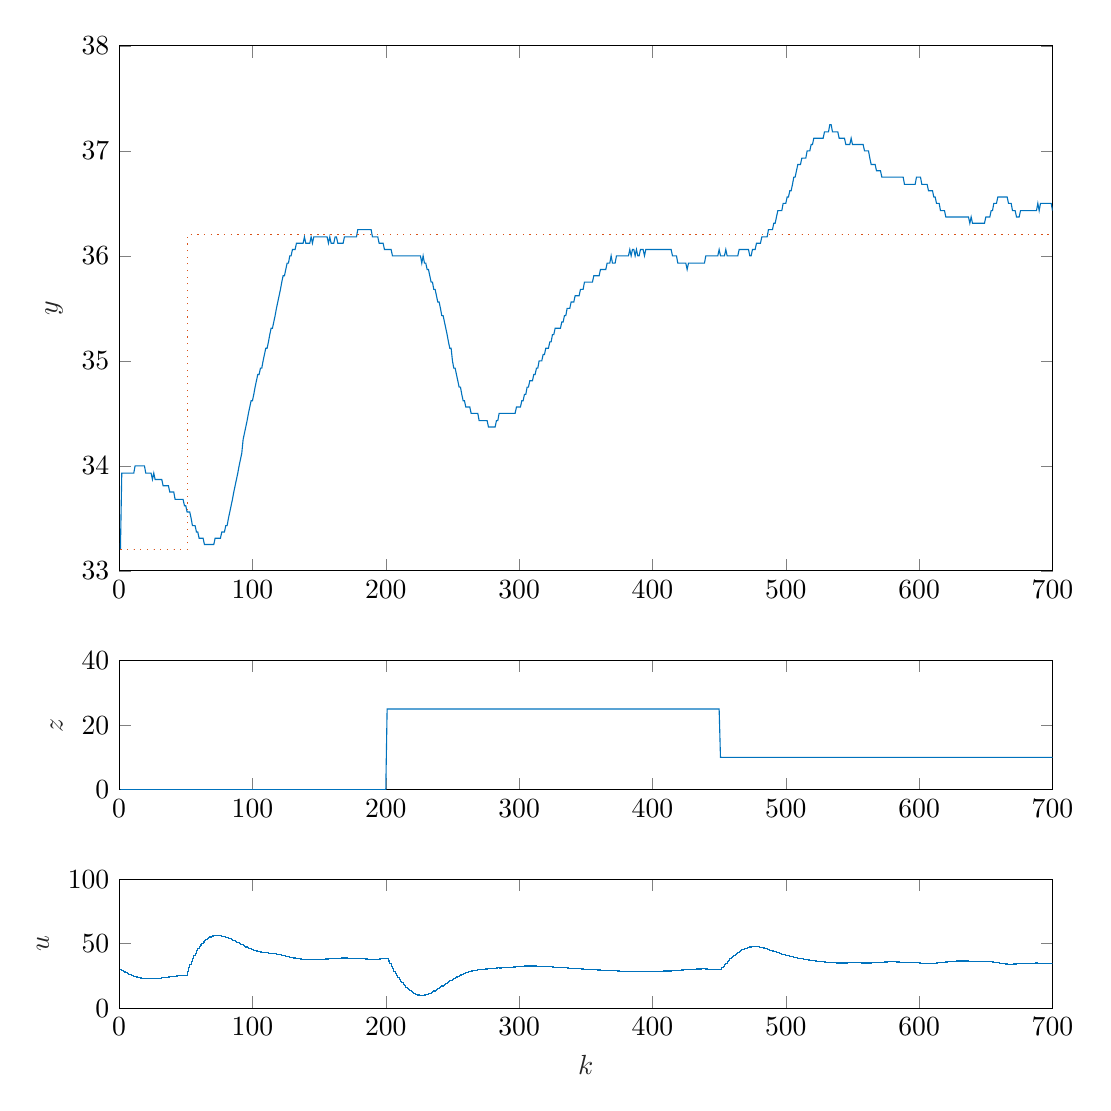
\begin{tikzpicture}

\begin{axis}[%
width=4.667in,
height=0.645in,
at={(0.583in,0.52in)},
scale only axis,
xmin=0,
xmax=700,
xtick={0,100,200,300,400,500,600,700},
xlabel style={font=\color{white!15!black}},
xlabel={$k$},
ymin=0,
ymax=100,
ytick={0,50,100},
ylabel style={font=\color{white!15!black}},
ylabel={$u$},
axis background/.style={fill=white}
]
\addplot[const plot, color=mycolor1, forget plot] table[row sep=crcr] {%
1	30\\
2	29.295\\
3	28.637\\
4	28.027\\
5	27.461\\
6	26.938\\
7	26.456\\
8	26.014\\
9	25.61\\
10	25.242\\
11	24.908\\
12	24.54\\
13	24.208\\
14	23.91\\
15	23.644\\
16	23.409\\
17	23.203\\
18	23.025\\
19	22.872\\
20	22.811\\
21	22.769\\
22	22.744\\
23	22.735\\
24	22.74\\
25	22.817\\
26	22.844\\
27	22.941\\
28	23.044\\
29	23.151\\
30	23.259\\
31	23.366\\
32	23.47\\
33	23.627\\
34	23.775\\
35	23.911\\
36	24.036\\
37	24.149\\
38	24.307\\
39	24.447\\
40	24.571\\
41	24.678\\
42	24.835\\
43	24.971\\
44	25.087\\
45	25.182\\
46	25.259\\
47	25.318\\
48	25.359\\
49	25.443\\
50	25.508\\
51	28.512\\
52	31.299\\
53	33.875\\
54	36.308\\
55	38.613\\
56	40.725\\
57	42.653\\
58	44.464\\
59	46.105\\
60	47.641\\
61	49.02\\
62	50.249\\
63	51.338\\
64	52.351\\
65	53.234\\
66	53.996\\
67	54.643\\
68	55.183\\
69	55.623\\
70	55.969\\
71	56.228\\
72	56.348\\
73	56.397\\
74	56.38\\
75	56.303\\
76	56.171\\
77	55.929\\
78	55.655\\
79	55.359\\
80	54.993\\
81	54.628\\
82	54.205\\
83	53.744\\
84	53.255\\
85	52.746\\
86	52.215\\
87	51.678\\
88	51.141\\
89	50.608\\
90	50.074\\
91	49.552\\
92	49.045\\
93	48.488\\
94	47.953\\
95	47.442\\
96	46.955\\
97	46.482\\
98	46.034\\
99	45.61\\
100	45.266\\
101	44.94\\
102	44.62\\
103	44.316\\
104	44.026\\
105	43.806\\
106	43.593\\
107	43.443\\
108	43.283\\
109	43.122\\
110	42.959\\
111	42.85\\
112	42.731\\
113	42.593\\
114	42.444\\
115	42.341\\
116	42.221\\
117	42.085\\
118	41.922\\
119	41.741\\
120	41.542\\
121	41.326\\
122	41.082\\
123	40.821\\
124	40.6\\
125	40.359\\
126	40.097\\
127	39.872\\
128	39.615\\
129	39.395\\
130	39.15\\
131	38.939\\
132	38.761\\
133	38.553\\
134	38.377\\
135	38.23\\
136	38.109\\
137	38.013\\
138	37.939\\
139	37.827\\
140	37.797\\
141	37.783\\
142	37.785\\
143	37.801\\
144	37.771\\
145	37.813\\
146	37.807\\
147	37.813\\
148	37.829\\
149	37.854\\
150	37.885\\
151	37.923\\
152	37.965\\
153	38.011\\
154	38.058\\
155	38.107\\
156	38.157\\
157	38.263\\
158	38.307\\
159	38.407\\
160	38.5\\
161	38.587\\
162	38.609\\
163	38.628\\
164	38.702\\
165	38.769\\
166	38.829\\
167	38.882\\
168	38.929\\
169	38.912\\
170	38.893\\
171	38.873\\
172	38.851\\
173	38.828\\
174	38.804\\
175	38.779\\
176	38.753\\
177	38.727\\
178	38.701\\
179	38.608\\
180	38.519\\
181	38.435\\
182	38.356\\
183	38.282\\
184	38.213\\
185	38.149\\
186	38.09\\
187	38.037\\
188	37.988\\
189	37.945\\
190	37.974\\
191	38.003\\
192	38.032\\
193	38.062\\
194	38.092\\
195	38.18\\
196	38.265\\
197	38.345\\
198	38.422\\
199	38.553\\
200	38.676\\
201	38.792\\
202	36.583\\
203	34.467\\
204	32.442\\
205	30.566\\
206	28.774\\
207	27.067\\
208	25.441\\
209	23.896\\
210	22.429\\
211	21.04\\
212	19.725\\
213	18.484\\
214	17.314\\
215	16.213\\
216	15.185\\
217	14.239\\
218	13.381\\
219	12.616\\
220	11.946\\
221	11.372\\
222	10.895\\
223	10.513\\
224	10.225\\
225	10.028\\
226	9.9186\\
227	9.9619\\
228	10.014\\
229	10.204\\
230	10.449\\
231	10.798\\
232	11.179\\
233	11.645\\
234	12.182\\
235	12.722\\
236	13.328\\
237	13.922\\
238	14.557\\
239	15.226\\
240	15.863\\
241	16.524\\
242	17.211\\
243	17.852\\
244	18.503\\
245	19.16\\
246	19.819\\
247	20.485\\
248	21.147\\
249	21.743\\
250	22.392\\
251	23.04\\
252	23.618\\
253	24.186\\
254	24.745\\
255	25.294\\
256	25.777\\
257	26.264\\
258	26.746\\
259	27.167\\
260	27.588\\
261	27.953\\
262	28.266\\
263	28.532\\
264	28.815\\
265	29.055\\
266	29.259\\
267	29.429\\
268	29.571\\
269	29.687\\
270	29.849\\
271	29.988\\
272	30.108\\
273	30.211\\
274	30.301\\
275	30.38\\
276	30.45\\
277	30.573\\
278	30.688\\
279	30.797\\
280	30.903\\
281	31.007\\
282	31.11\\
283	31.156\\
284	31.208\\
285	31.2\\
286	31.204\\
287	31.221\\
288	31.251\\
289	31.294\\
290	31.35\\
291	31.42\\
292	31.501\\
293	31.595\\
294	31.7\\
295	31.816\\
296	31.942\\
297	32.077\\
298	32.164\\
299	32.263\\
300	32.373\\
301	32.494\\
302	32.567\\
303	32.652\\
304	32.691\\
305	32.746\\
306	32.747\\
307	32.765\\
308	32.742\\
309	32.738\\
310	32.753\\
311	32.726\\
312	32.718\\
313	32.67\\
314	32.642\\
315	32.566\\
316	32.511\\
317	32.477\\
318	32.404\\
319	32.353\\
320	32.264\\
321	32.199\\
322	32.156\\
323	32.075\\
324	32.017\\
325	31.914\\
326	31.836\\
327	31.723\\
328	31.637\\
329	31.575\\
330	31.537\\
331	31.519\\
332	31.464\\
333	31.429\\
334	31.355\\
335	31.303\\
336	31.202\\
337	31.123\\
338	31.064\\
339	30.966\\
340	30.887\\
341	30.828\\
342	30.727\\
343	30.645\\
344	30.581\\
345	30.533\\
346	30.441\\
347	30.367\\
348	30.308\\
349	30.195\\
350	30.1\\
351	30.022\\
352	29.958\\
353	29.908\\
354	29.87\\
355	29.843\\
356	29.769\\
357	29.708\\
358	29.659\\
359	29.622\\
360	29.595\\
361	29.52\\
362	29.458\\
363	29.408\\
364	29.369\\
365	29.339\\
366	29.261\\
367	29.196\\
368	29.141\\
369	29.03\\
370	29\\
371	28.98\\
372	28.967\\
373	28.894\\
374	28.833\\
375	28.781\\
376	28.74\\
377	28.707\\
378	28.682\\
379	28.665\\
380	28.654\\
381	28.649\\
382	28.651\\
383	28.599\\
384	28.614\\
385	28.575\\
386	28.544\\
387	28.577\\
388	28.555\\
389	28.597\\
390	28.639\\
391	28.626\\
392	28.616\\
393	28.611\\
394	28.668\\
395	28.666\\
396	28.667\\
397	28.67\\
398	28.676\\
399	28.683\\
400	28.692\\
401	28.703\\
402	28.715\\
403	28.728\\
404	28.741\\
405	28.756\\
406	28.77\\
407	28.785\\
408	28.8\\
409	28.816\\
410	28.832\\
411	28.848\\
412	28.864\\
413	28.879\\
414	28.895\\
415	28.969\\
416	29.038\\
417	29.104\\
418	29.165\\
419	29.291\\
420	29.409\\
421	29.518\\
422	29.62\\
423	29.715\\
424	29.803\\
425	29.883\\
426	30.016\\
427	30.08\\
428	30.138\\
429	30.19\\
430	30.237\\
431	30.279\\
432	30.316\\
433	30.349\\
434	30.377\\
435	30.402\\
436	30.422\\
437	30.439\\
438	30.452\\
439	30.463\\
440	30.402\\
441	30.344\\
442	30.287\\
443	30.232\\
444	30.18\\
445	30.131\\
446	30.084\\
447	30.039\\
448	29.998\\
449	29.961\\
450	29.868\\
451	29.841\\
452	31.207\\
453	32.517\\
454	33.771\\
455	34.911\\
456	36.06\\
457	37.154\\
458	38.196\\
459	39.186\\
460	40.126\\
461	41.016\\
462	41.857\\
463	42.651\\
464	43.4\\
465	44.046\\
466	44.649\\
467	45.203\\
468	45.706\\
469	46.153\\
470	46.544\\
471	46.878\\
472	47.154\\
473	47.431\\
474	47.65\\
475	47.752\\
476	47.803\\
477	47.804\\
478	47.699\\
479	47.558\\
480	47.386\\
481	47.19\\
482	46.915\\
483	46.627\\
484	46.332\\
485	46.032\\
486	45.733\\
487	45.371\\
488	45.02\\
489	44.685\\
490	44.366\\
491	44.009\\
492	43.677\\
493	43.312\\
494	42.92\\
495	42.563\\
496	42.241\\
497	41.953\\
498	41.631\\
499	41.347\\
500	41.1\\
501	40.83\\
502	40.597\\
503	40.343\\
504	40.126\\
505	39.887\\
506	39.616\\
507	39.385\\
508	39.131\\
509	38.856\\
510	38.62\\
511	38.418\\
512	38.19\\
513	37.995\\
514	37.83\\
515	37.692\\
516	37.511\\
517	37.357\\
518	37.226\\
519	37.058\\
520	36.914\\
521	36.731\\
522	36.571\\
523	36.43\\
524	36.307\\
525	36.199\\
526	36.106\\
527	36.024\\
528	35.954\\
529	35.834\\
530	35.727\\
531	35.63\\
532	35.542\\
533	35.394\\
534	35.258\\
535	35.2\\
536	35.146\\
537	35.096\\
538	35.047\\
539	35.001\\
540	35.014\\
541	35.023\\
542	35.029\\
543	35.031\\
544	35.029\\
545	35.08\\
546	35.124\\
547	35.159\\
548	35.186\\
549	35.146\\
550	35.161\\
551	35.167\\
552	35.166\\
553	35.157\\
554	35.141\\
555	35.119\\
556	35.09\\
557	35.054\\
558	35.013\\
559	35.024\\
560	35.026\\
561	35.018\\
562	35.002\\
563	35.045\\
564	35.134\\
565	35.207\\
566	35.266\\
567	35.311\\
568	35.402\\
569	35.477\\
570	35.536\\
571	35.582\\
572	35.673\\
573	35.749\\
574	35.809\\
575	35.856\\
576	35.89\\
577	35.912\\
578	35.923\\
579	35.923\\
580	35.914\\
581	35.896\\
582	35.869\\
583	35.835\\
584	35.794\\
585	35.746\\
586	35.692\\
587	35.633\\
588	35.57\\
589	35.569\\
590	35.561\\
591	35.545\\
592	35.523\\
593	35.495\\
594	35.462\\
595	35.425\\
596	35.384\\
597	35.34\\
598	35.226\\
599	35.115\\
600	35.006\\
601	34.902\\
602	34.868\\
603	34.833\\
604	34.798\\
605	34.763\\
606	34.727\\
607	34.748\\
608	34.766\\
609	34.78\\
610	34.791\\
611	34.856\\
612	34.913\\
613	35.021\\
614	35.119\\
615	35.206\\
616	35.351\\
617	35.481\\
618	35.599\\
619	35.703\\
620	35.854\\
621	35.989\\
622	36.109\\
623	36.215\\
624	36.307\\
625	36.387\\
626	36.453\\
627	36.508\\
628	36.551\\
629	36.583\\
630	36.605\\
631	36.617\\
632	36.621\\
633	36.615\\
634	36.602\\
635	36.582\\
636	36.556\\
637	36.524\\
638	36.545\\
639	36.5\\
640	36.509\\
641	36.512\\
642	36.508\\
643	36.5\\
644	36.488\\
645	36.473\\
646	36.454\\
647	36.434\\
648	36.412\\
649	36.389\\
650	36.309\\
651	36.232\\
652	36.159\\
653	36.09\\
654	35.968\\
655	35.855\\
656	35.681\\
657	35.521\\
658	35.372\\
659	35.178\\
660	34.998\\
661	34.833\\
662	34.682\\
663	34.544\\
664	34.418\\
665	34.305\\
666	34.203\\
667	34.17\\
668	34.143\\
669	34.122\\
670	34.174\\
671	34.227\\
672	34.28\\
673	34.392\\
674	34.499\\
675	34.602\\
676	34.643\\
677	34.683\\
678	34.723\\
679	34.762\\
680	34.8\\
681	34.836\\
682	34.871\\
683	34.903\\
684	34.933\\
685	34.959\\
686	34.982\\
687	35.002\\
688	35.018\\
689	34.961\\
690	34.973\\
691	34.913\\
692	34.853\\
693	34.794\\
694	34.734\\
695	34.675\\
696	34.616\\
697	34.558\\
698	34.501\\
699	34.446\\
700	34.459\\
};
\end{axis}

\begin{axis}[%
width=4.667in,
height=0.645in,
at={(0.583in,1.613in)},
scale only axis,
xmin=0,
xmax=700,
xtick={0,100,200,300,400,500,600,700},
ymin=0,
ymax=40,
ytick={0,20,40},
ylabel style={font=\color{white!15!black}},
ylabel={$z$},
axis background/.style={fill=white}
]
\addplot [color=mycolor1, forget plot]
  table[row sep=crcr]{%
1	0\\
2	0\\
3	0\\
4	0\\
5	0\\
6	0\\
7	0\\
8	0\\
9	0\\
10	0\\
11	0\\
12	0\\
13	0\\
14	0\\
15	0\\
16	0\\
17	0\\
18	0\\
19	0\\
20	0\\
21	0\\
22	0\\
23	0\\
24	0\\
25	0\\
26	0\\
27	0\\
28	0\\
29	0\\
30	0\\
31	0\\
32	0\\
33	0\\
34	0\\
35	0\\
36	0\\
37	0\\
38	0\\
39	0\\
40	0\\
41	0\\
42	0\\
43	0\\
44	0\\
45	0\\
46	0\\
47	0\\
48	0\\
49	0\\
50	0\\
51	0\\
52	0\\
53	0\\
54	0\\
55	0\\
56	0\\
57	0\\
58	0\\
59	0\\
60	0\\
61	0\\
62	0\\
63	0\\
64	0\\
65	0\\
66	0\\
67	0\\
68	0\\
69	0\\
70	0\\
71	0\\
72	0\\
73	0\\
74	0\\
75	0\\
76	0\\
77	0\\
78	0\\
79	0\\
80	0\\
81	0\\
82	0\\
83	0\\
84	0\\
85	0\\
86	0\\
87	0\\
88	0\\
89	0\\
90	0\\
91	0\\
92	0\\
93	0\\
94	0\\
95	0\\
96	0\\
97	0\\
98	0\\
99	0\\
100	0\\
101	0\\
102	0\\
103	0\\
104	0\\
105	0\\
106	0\\
107	0\\
108	0\\
109	0\\
110	0\\
111	0\\
112	0\\
113	0\\
114	0\\
115	0\\
116	0\\
117	0\\
118	0\\
119	0\\
120	0\\
121	0\\
122	0\\
123	0\\
124	0\\
125	0\\
126	0\\
127	0\\
128	0\\
129	0\\
130	0\\
131	0\\
132	0\\
133	0\\
134	0\\
135	0\\
136	0\\
137	0\\
138	0\\
139	0\\
140	0\\
141	0\\
142	0\\
143	0\\
144	0\\
145	0\\
146	0\\
147	0\\
148	0\\
149	0\\
150	0\\
151	0\\
152	0\\
153	0\\
154	0\\
155	0\\
156	0\\
157	0\\
158	0\\
159	0\\
160	0\\
161	0\\
162	0\\
163	0\\
164	0\\
165	0\\
166	0\\
167	0\\
168	0\\
169	0\\
170	0\\
171	0\\
172	0\\
173	0\\
174	0\\
175	0\\
176	0\\
177	0\\
178	0\\
179	0\\
180	0\\
181	0\\
182	0\\
183	0\\
184	0\\
185	0\\
186	0\\
187	0\\
188	0\\
189	0\\
190	0\\
191	0\\
192	0\\
193	0\\
194	0\\
195	0\\
196	0\\
197	0\\
198	0\\
199	0\\
200	0\\
201	25\\
202	25\\
203	25\\
204	25\\
205	25\\
206	25\\
207	25\\
208	25\\
209	25\\
210	25\\
211	25\\
212	25\\
213	25\\
214	25\\
215	25\\
216	25\\
217	25\\
218	25\\
219	25\\
220	25\\
221	25\\
222	25\\
223	25\\
224	25\\
225	25\\
226	25\\
227	25\\
228	25\\
229	25\\
230	25\\
231	25\\
232	25\\
233	25\\
234	25\\
235	25\\
236	25\\
237	25\\
238	25\\
239	25\\
240	25\\
241	25\\
242	25\\
243	25\\
244	25\\
245	25\\
246	25\\
247	25\\
248	25\\
249	25\\
250	25\\
251	25\\
252	25\\
253	25\\
254	25\\
255	25\\
256	25\\
257	25\\
258	25\\
259	25\\
260	25\\
261	25\\
262	25\\
263	25\\
264	25\\
265	25\\
266	25\\
267	25\\
268	25\\
269	25\\
270	25\\
271	25\\
272	25\\
273	25\\
274	25\\
275	25\\
276	25\\
277	25\\
278	25\\
279	25\\
280	25\\
281	25\\
282	25\\
283	25\\
284	25\\
285	25\\
286	25\\
287	25\\
288	25\\
289	25\\
290	25\\
291	25\\
292	25\\
293	25\\
294	25\\
295	25\\
296	25\\
297	25\\
298	25\\
299	25\\
300	25\\
301	25\\
302	25\\
303	25\\
304	25\\
305	25\\
306	25\\
307	25\\
308	25\\
309	25\\
310	25\\
311	25\\
312	25\\
313	25\\
314	25\\
315	25\\
316	25\\
317	25\\
318	25\\
319	25\\
320	25\\
321	25\\
322	25\\
323	25\\
324	25\\
325	25\\
326	25\\
327	25\\
328	25\\
329	25\\
330	25\\
331	25\\
332	25\\
333	25\\
334	25\\
335	25\\
336	25\\
337	25\\
338	25\\
339	25\\
340	25\\
341	25\\
342	25\\
343	25\\
344	25\\
345	25\\
346	25\\
347	25\\
348	25\\
349	25\\
350	25\\
351	25\\
352	25\\
353	25\\
354	25\\
355	25\\
356	25\\
357	25\\
358	25\\
359	25\\
360	25\\
361	25\\
362	25\\
363	25\\
364	25\\
365	25\\
366	25\\
367	25\\
368	25\\
369	25\\
370	25\\
371	25\\
372	25\\
373	25\\
374	25\\
375	25\\
376	25\\
377	25\\
378	25\\
379	25\\
380	25\\
381	25\\
382	25\\
383	25\\
384	25\\
385	25\\
386	25\\
387	25\\
388	25\\
389	25\\
390	25\\
391	25\\
392	25\\
393	25\\
394	25\\
395	25\\
396	25\\
397	25\\
398	25\\
399	25\\
400	25\\
401	25\\
402	25\\
403	25\\
404	25\\
405	25\\
406	25\\
407	25\\
408	25\\
409	25\\
410	25\\
411	25\\
412	25\\
413	25\\
414	25\\
415	25\\
416	25\\
417	25\\
418	25\\
419	25\\
420	25\\
421	25\\
422	25\\
423	25\\
424	25\\
425	25\\
426	25\\
427	25\\
428	25\\
429	25\\
430	25\\
431	25\\
432	25\\
433	25\\
434	25\\
435	25\\
436	25\\
437	25\\
438	25\\
439	25\\
440	25\\
441	25\\
442	25\\
443	25\\
444	25\\
445	25\\
446	25\\
447	25\\
448	25\\
449	25\\
450	25\\
451	10\\
452	10\\
453	10\\
454	10\\
455	10\\
456	10\\
457	10\\
458	10\\
459	10\\
460	10\\
461	10\\
462	10\\
463	10\\
464	10\\
465	10\\
466	10\\
467	10\\
468	10\\
469	10\\
470	10\\
471	10\\
472	10\\
473	10\\
474	10\\
475	10\\
476	10\\
477	10\\
478	10\\
479	10\\
480	10\\
481	10\\
482	10\\
483	10\\
484	10\\
485	10\\
486	10\\
487	10\\
488	10\\
489	10\\
490	10\\
491	10\\
492	10\\
493	10\\
494	10\\
495	10\\
496	10\\
497	10\\
498	10\\
499	10\\
500	10\\
501	10\\
502	10\\
503	10\\
504	10\\
505	10\\
506	10\\
507	10\\
508	10\\
509	10\\
510	10\\
511	10\\
512	10\\
513	10\\
514	10\\
515	10\\
516	10\\
517	10\\
518	10\\
519	10\\
520	10\\
521	10\\
522	10\\
523	10\\
524	10\\
525	10\\
526	10\\
527	10\\
528	10\\
529	10\\
530	10\\
531	10\\
532	10\\
533	10\\
534	10\\
535	10\\
536	10\\
537	10\\
538	10\\
539	10\\
540	10\\
541	10\\
542	10\\
543	10\\
544	10\\
545	10\\
546	10\\
547	10\\
548	10\\
549	10\\
550	10\\
551	10\\
552	10\\
553	10\\
554	10\\
555	10\\
556	10\\
557	10\\
558	10\\
559	10\\
560	10\\
561	10\\
562	10\\
563	10\\
564	10\\
565	10\\
566	10\\
567	10\\
568	10\\
569	10\\
570	10\\
571	10\\
572	10\\
573	10\\
574	10\\
575	10\\
576	10\\
577	10\\
578	10\\
579	10\\
580	10\\
581	10\\
582	10\\
583	10\\
584	10\\
585	10\\
586	10\\
587	10\\
588	10\\
589	10\\
590	10\\
591	10\\
592	10\\
593	10\\
594	10\\
595	10\\
596	10\\
597	10\\
598	10\\
599	10\\
600	10\\
601	10\\
602	10\\
603	10\\
604	10\\
605	10\\
606	10\\
607	10\\
608	10\\
609	10\\
610	10\\
611	10\\
612	10\\
613	10\\
614	10\\
615	10\\
616	10\\
617	10\\
618	10\\
619	10\\
620	10\\
621	10\\
622	10\\
623	10\\
624	10\\
625	10\\
626	10\\
627	10\\
628	10\\
629	10\\
630	10\\
631	10\\
632	10\\
633	10\\
634	10\\
635	10\\
636	10\\
637	10\\
638	10\\
639	10\\
640	10\\
641	10\\
642	10\\
643	10\\
644	10\\
645	10\\
646	10\\
647	10\\
648	10\\
649	10\\
650	10\\
651	10\\
652	10\\
653	10\\
654	10\\
655	10\\
656	10\\
657	10\\
658	10\\
659	10\\
660	10\\
661	10\\
662	10\\
663	10\\
664	10\\
665	10\\
666	10\\
667	10\\
668	10\\
669	10\\
670	10\\
671	10\\
672	10\\
673	10\\
674	10\\
675	10\\
676	10\\
677	10\\
678	10\\
679	10\\
680	10\\
681	10\\
682	10\\
683	10\\
684	10\\
685	10\\
686	10\\
687	10\\
688	10\\
689	10\\
690	10\\
691	10\\
692	10\\
693	10\\
694	10\\
695	10\\
696	10\\
697	10\\
698	10\\
699	10\\
700	10\\
};
\end{axis}

\begin{axis}[%
width=4.667in,
height=2.625in,
at={(0.583in,2.707in)},
scale only axis,
xmin=0,
xmax=700,
xtick={0,100,200,300,400,500,600,700},
ymin=33,
ymax=38,
ytick={33,34,35,36,37,38},
ylabel style={font=\color{white!15!black}},
ylabel={$y$},
axis background/.style={fill=white}
]
\addplot [color=mycolor1, forget plot]
  table[row sep=crcr]{%
1	33.2\\
2	33.93\\
3	33.93\\
4	33.93\\
5	33.93\\
6	33.93\\
7	33.93\\
8	33.93\\
9	33.93\\
10	33.93\\
11	33.93\\
12	34\\
13	34\\
14	34\\
15	34\\
16	34\\
17	34\\
18	34\\
19	34\\
20	33.93\\
21	33.93\\
22	33.93\\
23	33.93\\
24	33.93\\
25	33.87\\
26	33.93\\
27	33.87\\
28	33.87\\
29	33.87\\
30	33.87\\
31	33.87\\
32	33.87\\
33	33.81\\
34	33.81\\
35	33.81\\
36	33.81\\
37	33.81\\
38	33.75\\
39	33.75\\
40	33.75\\
41	33.75\\
42	33.68\\
43	33.68\\
44	33.68\\
45	33.68\\
46	33.68\\
47	33.68\\
48	33.68\\
49	33.62\\
50	33.62\\
51	33.56\\
52	33.56\\
53	33.56\\
54	33.5\\
55	33.43\\
56	33.43\\
57	33.43\\
58	33.37\\
59	33.37\\
60	33.31\\
61	33.31\\
62	33.31\\
63	33.31\\
64	33.25\\
65	33.25\\
66	33.25\\
67	33.25\\
68	33.25\\
69	33.25\\
70	33.25\\
71	33.25\\
72	33.31\\
73	33.31\\
74	33.31\\
75	33.31\\
76	33.31\\
77	33.37\\
78	33.37\\
79	33.37\\
80	33.43\\
81	33.43\\
82	33.5\\
83	33.56\\
84	33.62\\
85	33.68\\
86	33.75\\
87	33.81\\
88	33.87\\
89	33.93\\
90	34\\
91	34.06\\
92	34.12\\
93	34.25\\
94	34.31\\
95	34.37\\
96	34.43\\
97	34.5\\
98	34.56\\
99	34.62\\
100	34.62\\
101	34.68\\
102	34.75\\
103	34.81\\
104	34.87\\
105	34.87\\
106	34.93\\
107	34.93\\
108	35\\
109	35.06\\
110	35.12\\
111	35.12\\
112	35.18\\
113	35.25\\
114	35.31\\
115	35.31\\
116	35.37\\
117	35.43\\
118	35.5\\
119	35.56\\
120	35.62\\
121	35.68\\
122	35.75\\
123	35.81\\
124	35.81\\
125	35.87\\
126	35.93\\
127	35.93\\
128	36\\
129	36\\
130	36.06\\
131	36.06\\
132	36.06\\
133	36.12\\
134	36.12\\
135	36.12\\
136	36.12\\
137	36.12\\
138	36.12\\
139	36.18\\
140	36.12\\
141	36.12\\
142	36.12\\
143	36.12\\
144	36.18\\
145	36.12\\
146	36.18\\
147	36.18\\
148	36.18\\
149	36.18\\
150	36.18\\
151	36.18\\
152	36.18\\
153	36.18\\
154	36.18\\
155	36.18\\
156	36.18\\
157	36.12\\
158	36.18\\
159	36.12\\
160	36.12\\
161	36.12\\
162	36.18\\
163	36.18\\
164	36.12\\
165	36.12\\
166	36.12\\
167	36.12\\
168	36.12\\
169	36.18\\
170	36.18\\
171	36.18\\
172	36.18\\
173	36.18\\
174	36.18\\
175	36.18\\
176	36.18\\
177	36.18\\
178	36.18\\
179	36.25\\
180	36.25\\
181	36.25\\
182	36.25\\
183	36.25\\
184	36.25\\
185	36.25\\
186	36.25\\
187	36.25\\
188	36.25\\
189	36.25\\
190	36.18\\
191	36.18\\
192	36.18\\
193	36.18\\
194	36.18\\
195	36.12\\
196	36.12\\
197	36.12\\
198	36.12\\
199	36.06\\
200	36.06\\
201	36.06\\
202	36.06\\
203	36.06\\
204	36.06\\
205	36\\
206	36\\
207	36\\
208	36\\
209	36\\
210	36\\
211	36\\
212	36\\
213	36\\
214	36\\
215	36\\
216	36\\
217	36\\
218	36\\
219	36\\
220	36\\
221	36\\
222	36\\
223	36\\
224	36\\
225	36\\
226	36\\
227	35.93\\
228	36\\
229	35.93\\
230	35.93\\
231	35.87\\
232	35.87\\
233	35.81\\
234	35.75\\
235	35.75\\
236	35.68\\
237	35.68\\
238	35.62\\
239	35.56\\
240	35.56\\
241	35.5\\
242	35.43\\
243	35.43\\
244	35.37\\
245	35.31\\
246	35.25\\
247	35.18\\
248	35.12\\
249	35.12\\
250	35\\
251	34.93\\
252	34.93\\
253	34.87\\
254	34.81\\
255	34.75\\
256	34.75\\
257	34.68\\
258	34.62\\
259	34.62\\
260	34.56\\
261	34.56\\
262	34.56\\
263	34.56\\
264	34.5\\
265	34.5\\
266	34.5\\
267	34.5\\
268	34.5\\
269	34.5\\
270	34.43\\
271	34.43\\
272	34.43\\
273	34.43\\
274	34.43\\
275	34.43\\
276	34.43\\
277	34.37\\
278	34.37\\
279	34.37\\
280	34.37\\
281	34.37\\
282	34.37\\
283	34.43\\
284	34.43\\
285	34.5\\
286	34.5\\
287	34.5\\
288	34.5\\
289	34.5\\
290	34.5\\
291	34.5\\
292	34.5\\
293	34.5\\
294	34.5\\
295	34.5\\
296	34.5\\
297	34.5\\
298	34.56\\
299	34.56\\
300	34.56\\
301	34.56\\
302	34.62\\
303	34.62\\
304	34.68\\
305	34.68\\
306	34.75\\
307	34.75\\
308	34.81\\
309	34.81\\
310	34.81\\
311	34.87\\
312	34.87\\
313	34.93\\
314	34.93\\
315	35\\
316	35\\
317	35\\
318	35.06\\
319	35.06\\
320	35.12\\
321	35.12\\
322	35.12\\
323	35.18\\
324	35.18\\
325	35.25\\
326	35.25\\
327	35.31\\
328	35.31\\
329	35.31\\
330	35.31\\
331	35.31\\
332	35.37\\
333	35.37\\
334	35.43\\
335	35.43\\
336	35.5\\
337	35.5\\
338	35.5\\
339	35.56\\
340	35.56\\
341	35.56\\
342	35.62\\
343	35.62\\
344	35.62\\
345	35.62\\
346	35.68\\
347	35.68\\
348	35.68\\
349	35.75\\
350	35.75\\
351	35.75\\
352	35.75\\
353	35.75\\
354	35.75\\
355	35.75\\
356	35.81\\
357	35.81\\
358	35.81\\
359	35.81\\
360	35.81\\
361	35.87\\
362	35.87\\
363	35.87\\
364	35.87\\
365	35.87\\
366	35.93\\
367	35.93\\
368	35.93\\
369	36\\
370	35.93\\
371	35.93\\
372	35.93\\
373	36\\
374	36\\
375	36\\
376	36\\
377	36\\
378	36\\
379	36\\
380	36\\
381	36\\
382	36\\
383	36.06\\
384	36\\
385	36.06\\
386	36.06\\
387	36\\
388	36.06\\
389	36\\
390	36\\
391	36.06\\
392	36.06\\
393	36.06\\
394	36\\
395	36.06\\
396	36.06\\
397	36.06\\
398	36.06\\
399	36.06\\
400	36.06\\
401	36.06\\
402	36.06\\
403	36.06\\
404	36.06\\
405	36.06\\
406	36.06\\
407	36.06\\
408	36.06\\
409	36.06\\
410	36.06\\
411	36.06\\
412	36.06\\
413	36.06\\
414	36.06\\
415	36\\
416	36\\
417	36\\
418	36\\
419	35.93\\
420	35.93\\
421	35.93\\
422	35.93\\
423	35.93\\
424	35.93\\
425	35.93\\
426	35.87\\
427	35.93\\
428	35.93\\
429	35.93\\
430	35.93\\
431	35.93\\
432	35.93\\
433	35.93\\
434	35.93\\
435	35.93\\
436	35.93\\
437	35.93\\
438	35.93\\
439	35.93\\
440	36\\
441	36\\
442	36\\
443	36\\
444	36\\
445	36\\
446	36\\
447	36\\
448	36\\
449	36\\
450	36.06\\
451	36\\
452	36\\
453	36\\
454	36\\
455	36.06\\
456	36\\
457	36\\
458	36\\
459	36\\
460	36\\
461	36\\
462	36\\
463	36\\
464	36\\
465	36.06\\
466	36.06\\
467	36.06\\
468	36.06\\
469	36.06\\
470	36.06\\
471	36.06\\
472	36.06\\
473	36\\
474	36\\
475	36.06\\
476	36.06\\
477	36.06\\
478	36.12\\
479	36.12\\
480	36.12\\
481	36.12\\
482	36.18\\
483	36.18\\
484	36.18\\
485	36.18\\
486	36.18\\
487	36.25\\
488	36.25\\
489	36.25\\
490	36.25\\
491	36.31\\
492	36.31\\
493	36.37\\
494	36.43\\
495	36.43\\
496	36.43\\
497	36.43\\
498	36.5\\
499	36.5\\
500	36.5\\
501	36.56\\
502	36.56\\
503	36.62\\
504	36.62\\
505	36.68\\
506	36.75\\
507	36.75\\
508	36.81\\
509	36.87\\
510	36.87\\
511	36.87\\
512	36.93\\
513	36.93\\
514	36.93\\
515	36.93\\
516	37\\
517	37\\
518	37\\
519	37.06\\
520	37.06\\
521	37.12\\
522	37.12\\
523	37.12\\
524	37.12\\
525	37.12\\
526	37.12\\
527	37.12\\
528	37.12\\
529	37.18\\
530	37.18\\
531	37.18\\
532	37.18\\
533	37.25\\
534	37.25\\
535	37.18\\
536	37.18\\
537	37.18\\
538	37.18\\
539	37.18\\
540	37.12\\
541	37.12\\
542	37.12\\
543	37.12\\
544	37.12\\
545	37.06\\
546	37.06\\
547	37.06\\
548	37.06\\
549	37.12\\
550	37.06\\
551	37.06\\
552	37.06\\
553	37.06\\
554	37.06\\
555	37.06\\
556	37.06\\
557	37.06\\
558	37.06\\
559	37\\
560	37\\
561	37\\
562	37\\
563	36.93\\
564	36.87\\
565	36.87\\
566	36.87\\
567	36.87\\
568	36.81\\
569	36.81\\
570	36.81\\
571	36.81\\
572	36.75\\
573	36.75\\
574	36.75\\
575	36.75\\
576	36.75\\
577	36.75\\
578	36.75\\
579	36.75\\
580	36.75\\
581	36.75\\
582	36.75\\
583	36.75\\
584	36.75\\
585	36.75\\
586	36.75\\
587	36.75\\
588	36.75\\
589	36.68\\
590	36.68\\
591	36.68\\
592	36.68\\
593	36.68\\
594	36.68\\
595	36.68\\
596	36.68\\
597	36.68\\
598	36.75\\
599	36.75\\
600	36.75\\
601	36.75\\
602	36.68\\
603	36.68\\
604	36.68\\
605	36.68\\
606	36.68\\
607	36.62\\
608	36.62\\
609	36.62\\
610	36.62\\
611	36.56\\
612	36.56\\
613	36.5\\
614	36.5\\
615	36.5\\
616	36.43\\
617	36.43\\
618	36.43\\
619	36.43\\
620	36.37\\
621	36.37\\
622	36.37\\
623	36.37\\
624	36.37\\
625	36.37\\
626	36.37\\
627	36.37\\
628	36.37\\
629	36.37\\
630	36.37\\
631	36.37\\
632	36.37\\
633	36.37\\
634	36.37\\
635	36.37\\
636	36.37\\
637	36.37\\
638	36.31\\
639	36.37\\
640	36.31\\
641	36.31\\
642	36.31\\
643	36.31\\
644	36.31\\
645	36.31\\
646	36.31\\
647	36.31\\
648	36.31\\
649	36.31\\
650	36.37\\
651	36.37\\
652	36.37\\
653	36.37\\
654	36.43\\
655	36.43\\
656	36.5\\
657	36.5\\
658	36.5\\
659	36.56\\
660	36.56\\
661	36.56\\
662	36.56\\
663	36.56\\
664	36.56\\
665	36.56\\
666	36.56\\
667	36.5\\
668	36.5\\
669	36.5\\
670	36.43\\
671	36.43\\
672	36.43\\
673	36.37\\
674	36.37\\
675	36.37\\
676	36.43\\
677	36.43\\
678	36.43\\
679	36.43\\
680	36.43\\
681	36.43\\
682	36.43\\
683	36.43\\
684	36.43\\
685	36.43\\
686	36.43\\
687	36.43\\
688	36.43\\
689	36.5\\
690	36.43\\
691	36.5\\
692	36.5\\
693	36.5\\
694	36.5\\
695	36.5\\
696	36.5\\
697	36.5\\
698	36.5\\
699	36.5\\
700	36.43\\
};
\addplot[const plot, color=mycolor2, dotted, forget plot] table[row sep=crcr] {%
1	33.2\\
2	33.2\\
3	33.2\\
4	33.2\\
5	33.2\\
6	33.2\\
7	33.2\\
8	33.2\\
9	33.2\\
10	33.2\\
11	33.2\\
12	33.2\\
13	33.2\\
14	33.2\\
15	33.2\\
16	33.2\\
17	33.2\\
18	33.2\\
19	33.2\\
20	33.2\\
21	33.2\\
22	33.2\\
23	33.2\\
24	33.2\\
25	33.2\\
26	33.2\\
27	33.2\\
28	33.2\\
29	33.2\\
30	33.2\\
31	33.2\\
32	33.2\\
33	33.2\\
34	33.2\\
35	33.2\\
36	33.2\\
37	33.2\\
38	33.2\\
39	33.2\\
40	33.2\\
41	33.2\\
42	33.2\\
43	33.2\\
44	33.2\\
45	33.2\\
46	33.2\\
47	33.2\\
48	33.2\\
49	33.2\\
50	33.2\\
51	36.2\\
52	36.2\\
53	36.2\\
54	36.2\\
55	36.2\\
56	36.2\\
57	36.2\\
58	36.2\\
59	36.2\\
60	36.2\\
61	36.2\\
62	36.2\\
63	36.2\\
64	36.2\\
65	36.2\\
66	36.2\\
67	36.2\\
68	36.2\\
69	36.2\\
70	36.2\\
71	36.2\\
72	36.2\\
73	36.2\\
74	36.2\\
75	36.2\\
76	36.2\\
77	36.2\\
78	36.2\\
79	36.2\\
80	36.2\\
81	36.2\\
82	36.2\\
83	36.2\\
84	36.2\\
85	36.2\\
86	36.2\\
87	36.2\\
88	36.2\\
89	36.2\\
90	36.2\\
91	36.2\\
92	36.2\\
93	36.2\\
94	36.2\\
95	36.2\\
96	36.2\\
97	36.2\\
98	36.2\\
99	36.2\\
100	36.2\\
101	36.2\\
102	36.2\\
103	36.2\\
104	36.2\\
105	36.2\\
106	36.2\\
107	36.2\\
108	36.2\\
109	36.2\\
110	36.2\\
111	36.2\\
112	36.2\\
113	36.2\\
114	36.2\\
115	36.2\\
116	36.2\\
117	36.2\\
118	36.2\\
119	36.2\\
120	36.2\\
121	36.2\\
122	36.2\\
123	36.2\\
124	36.2\\
125	36.2\\
126	36.2\\
127	36.2\\
128	36.2\\
129	36.2\\
130	36.2\\
131	36.2\\
132	36.2\\
133	36.2\\
134	36.2\\
135	36.2\\
136	36.2\\
137	36.2\\
138	36.2\\
139	36.2\\
140	36.2\\
141	36.2\\
142	36.2\\
143	36.2\\
144	36.2\\
145	36.2\\
146	36.2\\
147	36.2\\
148	36.2\\
149	36.2\\
150	36.2\\
151	36.2\\
152	36.2\\
153	36.2\\
154	36.2\\
155	36.2\\
156	36.2\\
157	36.2\\
158	36.2\\
159	36.2\\
160	36.2\\
161	36.2\\
162	36.2\\
163	36.2\\
164	36.2\\
165	36.2\\
166	36.2\\
167	36.2\\
168	36.2\\
169	36.2\\
170	36.2\\
171	36.2\\
172	36.2\\
173	36.2\\
174	36.2\\
175	36.2\\
176	36.2\\
177	36.2\\
178	36.2\\
179	36.2\\
180	36.2\\
181	36.2\\
182	36.2\\
183	36.2\\
184	36.2\\
185	36.2\\
186	36.2\\
187	36.2\\
188	36.2\\
189	36.2\\
190	36.2\\
191	36.2\\
192	36.2\\
193	36.2\\
194	36.2\\
195	36.2\\
196	36.2\\
197	36.2\\
198	36.2\\
199	36.2\\
200	36.2\\
201	36.2\\
202	36.2\\
203	36.2\\
204	36.2\\
205	36.2\\
206	36.2\\
207	36.2\\
208	36.2\\
209	36.2\\
210	36.2\\
211	36.2\\
212	36.2\\
213	36.2\\
214	36.2\\
215	36.2\\
216	36.2\\
217	36.2\\
218	36.2\\
219	36.2\\
220	36.2\\
221	36.2\\
222	36.2\\
223	36.2\\
224	36.2\\
225	36.2\\
226	36.2\\
227	36.2\\
228	36.2\\
229	36.2\\
230	36.2\\
231	36.2\\
232	36.2\\
233	36.2\\
234	36.2\\
235	36.2\\
236	36.2\\
237	36.2\\
238	36.2\\
239	36.2\\
240	36.2\\
241	36.2\\
242	36.2\\
243	36.2\\
244	36.2\\
245	36.2\\
246	36.2\\
247	36.2\\
248	36.2\\
249	36.2\\
250	36.2\\
251	36.2\\
252	36.2\\
253	36.2\\
254	36.2\\
255	36.2\\
256	36.2\\
257	36.2\\
258	36.2\\
259	36.2\\
260	36.2\\
261	36.2\\
262	36.2\\
263	36.2\\
264	36.2\\
265	36.2\\
266	36.2\\
267	36.2\\
268	36.2\\
269	36.2\\
270	36.2\\
271	36.2\\
272	36.2\\
273	36.2\\
274	36.2\\
275	36.2\\
276	36.2\\
277	36.2\\
278	36.2\\
279	36.2\\
280	36.2\\
281	36.2\\
282	36.2\\
283	36.2\\
284	36.2\\
285	36.2\\
286	36.2\\
287	36.2\\
288	36.2\\
289	36.2\\
290	36.2\\
291	36.2\\
292	36.2\\
293	36.2\\
294	36.2\\
295	36.2\\
296	36.2\\
297	36.2\\
298	36.2\\
299	36.2\\
300	36.2\\
301	36.2\\
302	36.2\\
303	36.2\\
304	36.2\\
305	36.2\\
306	36.2\\
307	36.2\\
308	36.2\\
309	36.2\\
310	36.2\\
311	36.2\\
312	36.2\\
313	36.2\\
314	36.2\\
315	36.2\\
316	36.2\\
317	36.2\\
318	36.2\\
319	36.2\\
320	36.2\\
321	36.2\\
322	36.2\\
323	36.2\\
324	36.2\\
325	36.2\\
326	36.2\\
327	36.2\\
328	36.2\\
329	36.2\\
330	36.2\\
331	36.2\\
332	36.2\\
333	36.2\\
334	36.2\\
335	36.2\\
336	36.2\\
337	36.2\\
338	36.2\\
339	36.2\\
340	36.2\\
341	36.2\\
342	36.2\\
343	36.2\\
344	36.2\\
345	36.2\\
346	36.2\\
347	36.2\\
348	36.2\\
349	36.2\\
350	36.2\\
351	36.2\\
352	36.2\\
353	36.2\\
354	36.2\\
355	36.2\\
356	36.2\\
357	36.2\\
358	36.2\\
359	36.2\\
360	36.2\\
361	36.2\\
362	36.2\\
363	36.2\\
364	36.2\\
365	36.2\\
366	36.2\\
367	36.2\\
368	36.2\\
369	36.2\\
370	36.2\\
371	36.2\\
372	36.2\\
373	36.2\\
374	36.2\\
375	36.2\\
376	36.2\\
377	36.2\\
378	36.2\\
379	36.2\\
380	36.2\\
381	36.2\\
382	36.2\\
383	36.2\\
384	36.2\\
385	36.2\\
386	36.2\\
387	36.2\\
388	36.2\\
389	36.2\\
390	36.2\\
391	36.2\\
392	36.2\\
393	36.2\\
394	36.2\\
395	36.2\\
396	36.2\\
397	36.2\\
398	36.2\\
399	36.2\\
400	36.2\\
401	36.2\\
402	36.2\\
403	36.2\\
404	36.2\\
405	36.2\\
406	36.2\\
407	36.2\\
408	36.2\\
409	36.2\\
410	36.2\\
411	36.2\\
412	36.2\\
413	36.2\\
414	36.2\\
415	36.2\\
416	36.2\\
417	36.2\\
418	36.2\\
419	36.2\\
420	36.2\\
421	36.2\\
422	36.2\\
423	36.2\\
424	36.2\\
425	36.2\\
426	36.2\\
427	36.2\\
428	36.2\\
429	36.2\\
430	36.2\\
431	36.2\\
432	36.2\\
433	36.2\\
434	36.2\\
435	36.2\\
436	36.2\\
437	36.2\\
438	36.2\\
439	36.2\\
440	36.2\\
441	36.2\\
442	36.2\\
443	36.2\\
444	36.2\\
445	36.2\\
446	36.2\\
447	36.2\\
448	36.2\\
449	36.2\\
450	36.2\\
451	36.2\\
452	36.2\\
453	36.2\\
454	36.2\\
455	36.2\\
456	36.2\\
457	36.2\\
458	36.2\\
459	36.2\\
460	36.2\\
461	36.2\\
462	36.2\\
463	36.2\\
464	36.2\\
465	36.2\\
466	36.2\\
467	36.2\\
468	36.2\\
469	36.2\\
470	36.2\\
471	36.2\\
472	36.2\\
473	36.2\\
474	36.2\\
475	36.2\\
476	36.2\\
477	36.2\\
478	36.2\\
479	36.2\\
480	36.2\\
481	36.2\\
482	36.2\\
483	36.2\\
484	36.2\\
485	36.2\\
486	36.2\\
487	36.2\\
488	36.2\\
489	36.2\\
490	36.2\\
491	36.2\\
492	36.2\\
493	36.2\\
494	36.2\\
495	36.2\\
496	36.2\\
497	36.2\\
498	36.2\\
499	36.2\\
500	36.2\\
501	36.2\\
502	36.2\\
503	36.2\\
504	36.2\\
505	36.2\\
506	36.2\\
507	36.2\\
508	36.2\\
509	36.2\\
510	36.2\\
511	36.2\\
512	36.2\\
513	36.2\\
514	36.2\\
515	36.2\\
516	36.2\\
517	36.2\\
518	36.2\\
519	36.2\\
520	36.2\\
521	36.2\\
522	36.2\\
523	36.2\\
524	36.2\\
525	36.2\\
526	36.2\\
527	36.2\\
528	36.2\\
529	36.2\\
530	36.2\\
531	36.2\\
532	36.2\\
533	36.2\\
534	36.2\\
535	36.2\\
536	36.2\\
537	36.2\\
538	36.2\\
539	36.2\\
540	36.2\\
541	36.2\\
542	36.2\\
543	36.2\\
544	36.2\\
545	36.2\\
546	36.2\\
547	36.2\\
548	36.2\\
549	36.2\\
550	36.2\\
551	36.2\\
552	36.2\\
553	36.2\\
554	36.2\\
555	36.2\\
556	36.2\\
557	36.2\\
558	36.2\\
559	36.2\\
560	36.2\\
561	36.2\\
562	36.2\\
563	36.2\\
564	36.2\\
565	36.2\\
566	36.2\\
567	36.2\\
568	36.2\\
569	36.2\\
570	36.2\\
571	36.2\\
572	36.2\\
573	36.2\\
574	36.2\\
575	36.2\\
576	36.2\\
577	36.2\\
578	36.2\\
579	36.2\\
580	36.2\\
581	36.2\\
582	36.2\\
583	36.2\\
584	36.2\\
585	36.2\\
586	36.2\\
587	36.2\\
588	36.2\\
589	36.2\\
590	36.2\\
591	36.2\\
592	36.2\\
593	36.2\\
594	36.2\\
595	36.2\\
596	36.2\\
597	36.2\\
598	36.2\\
599	36.2\\
600	36.2\\
601	36.2\\
602	36.2\\
603	36.2\\
604	36.2\\
605	36.2\\
606	36.2\\
607	36.2\\
608	36.2\\
609	36.2\\
610	36.2\\
611	36.2\\
612	36.2\\
613	36.2\\
614	36.2\\
615	36.2\\
616	36.2\\
617	36.2\\
618	36.2\\
619	36.2\\
620	36.2\\
621	36.2\\
622	36.2\\
623	36.2\\
624	36.2\\
625	36.2\\
626	36.2\\
627	36.2\\
628	36.2\\
629	36.2\\
630	36.2\\
631	36.2\\
632	36.2\\
633	36.2\\
634	36.2\\
635	36.2\\
636	36.2\\
637	36.2\\
638	36.2\\
639	36.2\\
640	36.2\\
641	36.2\\
642	36.2\\
643	36.2\\
644	36.2\\
645	36.2\\
646	36.2\\
647	36.2\\
648	36.2\\
649	36.2\\
650	36.2\\
651	36.2\\
652	36.2\\
653	36.2\\
654	36.2\\
655	36.2\\
656	36.2\\
657	36.2\\
658	36.2\\
659	36.2\\
660	36.2\\
661	36.2\\
662	36.2\\
663	36.2\\
664	36.2\\
665	36.2\\
666	36.2\\
667	36.2\\
668	36.2\\
669	36.2\\
670	36.2\\
671	36.2\\
672	36.2\\
673	36.2\\
674	36.2\\
675	36.2\\
676	36.2\\
677	36.2\\
678	36.2\\
679	36.2\\
680	36.2\\
681	36.2\\
682	36.2\\
683	36.2\\
684	36.2\\
685	36.2\\
686	36.2\\
687	36.2\\
688	36.2\\
689	36.2\\
690	36.2\\
691	36.2\\
692	36.2\\
693	36.2\\
694	36.2\\
695	36.2\\
696	36.2\\
697	36.2\\
698	36.2\\
699	36.2\\
700	36.2\\
};
\end{axis}
\end{tikzpicture}%
\caption{Regulacja DMC na obiekcie z pomiarem zakłóceń przy zastosowaniu błędnego modelu}
\label{R8}
\end{figure}
